\chapter{Introduction}\label{ch:introduction}

\section{Motivation}

Environmental concerns and the challenge to improve the livability of cities are key drivers in recent urban development. Especially in cities shaped by car-centric urbanism, the car is becoming increasingly problematic due to noise and air pollution as well as the narrowing of space required for parking. This issue is further amplified as more people inhabit cities. Electrifying traffic and making transportation more intelligent with cooperative transport systems is one important aspect of reducing these negative impacts and enhancing the livability of city centers \cite{seredynski_pathways_2023}. 

In parallel, an increasing number of cities are launching initiatives and pilot projects aimed at motivating more sustainable forms of mobility \cite{nieuwenhuijsen_car_2016}. A part of these projects focuses on making cycling more attractive. However, motivating more people to cycle is challenging due to two types of barriers: physical barriers and psychological barriers \cite{nieuwenhuijsen_implementing_2019}. Physical barriers relate to the expansion of cycling infrastructure, as well as supportive features such as bike rental stations and air stations. Psychological barriers involve attitudes and beliefs that hinder people from cycling. 

Since both types of barriers depend on each other, they can be considered a chicken-and-egg problem: to break down psychological barriers, barriers that physically obstruct cyclists must first be dismantled. However, this requires invasive changes to infrastructure and, consequently, citizen support. Thus, non-invasive solutions that improve the attitude towards cycling are highly desirable to accelerate the sustainable mobility transformation. A non-invasive approach involves making cycling smarter \cite{nikolaeva_smart_2019}. As traffic infrastructure and participants are increasingly networked with each other, new opportunities arise for digital solutions based on the communication of traffic-related data \cite{tran_factors_2023}.

Cities can provide digital solutions to cyclists that improve specific aspects of cycling as a complementary measure to other initiatives. One such solution is providing cyclists with a service through an app that ensures they reach a green traffic light. Known as Green Light Optimal Speed Advisory (GLOSA), this solution enables traffic participants to anticipate the switching behavior of upcoming traffic lights. Based on a prediction of these traffic lights, a speed advisory can be provided to the user. Applied to cyclists, such a solution has the potential to make cycling feel more intelligent and advantageous in general. Cyclists may choose to either accelerate and reach the green phase or conserve energy by coasting. In this manner, a GLOSA app may help cyclists reach their destination quicker or more comfortably.

Such a solution may not only be beneficial for cyclists but also for the city itself, collecting valuable data about cyclists' behaviors through the app. As part of a broader campaign, such an app may contribute to building a self-expanding cycling community. This is the challenge that Hamburg has set itself with the PrioBike project, named after the prioritization of bike mobility. Within this project, an app is to be created for Hamburg citizens that can be used free of charge and provides a GLOSA service. To support such a service, Hamburg provides real-time traffic light data for over 5,000 bike traffic lights through a centralized data broker. Based on this foundation, the main goal of this work is to realize and evaluate a GLOSA system for cyclists on the city scale. To accomplish this goal, existing solutions from the car-dominated research domain of GLOSA must be identified, and knowledge gaps for cyclist applications addressed. 

\section{Background}

Services similar to Green Light Optimal Speed Advisory were proposed as early as 2006. Back then, Sanchez et al. (2006) \cite{sanchez_predicting_2006} utilized the term "Intelligent Driver Model," showing how a system could be developed that helps drivers adapt to information from an upcoming traffic light. In 2008, Iglesias et al. \cite{iglesias_i2v_2008} proposed a perception-enhancing "Infrastructure to Vehicle Communication Driving Assistance System" that displays a traffic light's state to the driver, increasing the distance from which the traffic light's color can be seen. The idea of a "Green Wave App" recommending speeds to the user was first introduced by Otto and Hoyer (2010) \cite{otto_operating_2010}. In the same year, Tielert et al. \cite{tielert_impact_2010} introduced a "Traffic-Light-to-Vehicle-Communication" system. Then, in 2011, the term "ECO-Driving" or "ECO-Approach (and Departure)" was coined by Xia et al. (2011) \cite{xia_indirect_2011}, which would be reused over time by a few studies until today \cite{rakha_eco-driving_2011, rakha_aeris_2012, xia_field_2012, hao_eco-approach_2019, hu_lane-level_2023}. A few works in 2011 \cite{asadi_predictive_2011, raubitschek_predictive_2011} would also use the term "Predictive Cruise Control," referring to the prediction of the needed speed to pass the next traffic light at green. The first work that introduced the abbreviation GLOSA was published by Katsaros et al. in 2011 \cite{katsaros_performance_2011}, which has since become established in most studies.

\begin{figure}[t]
\centering
\resizebox{\linewidth}{!}{%
\begin{tabular}{p{0.45\linewidth}p{0.55\linewidth}}
  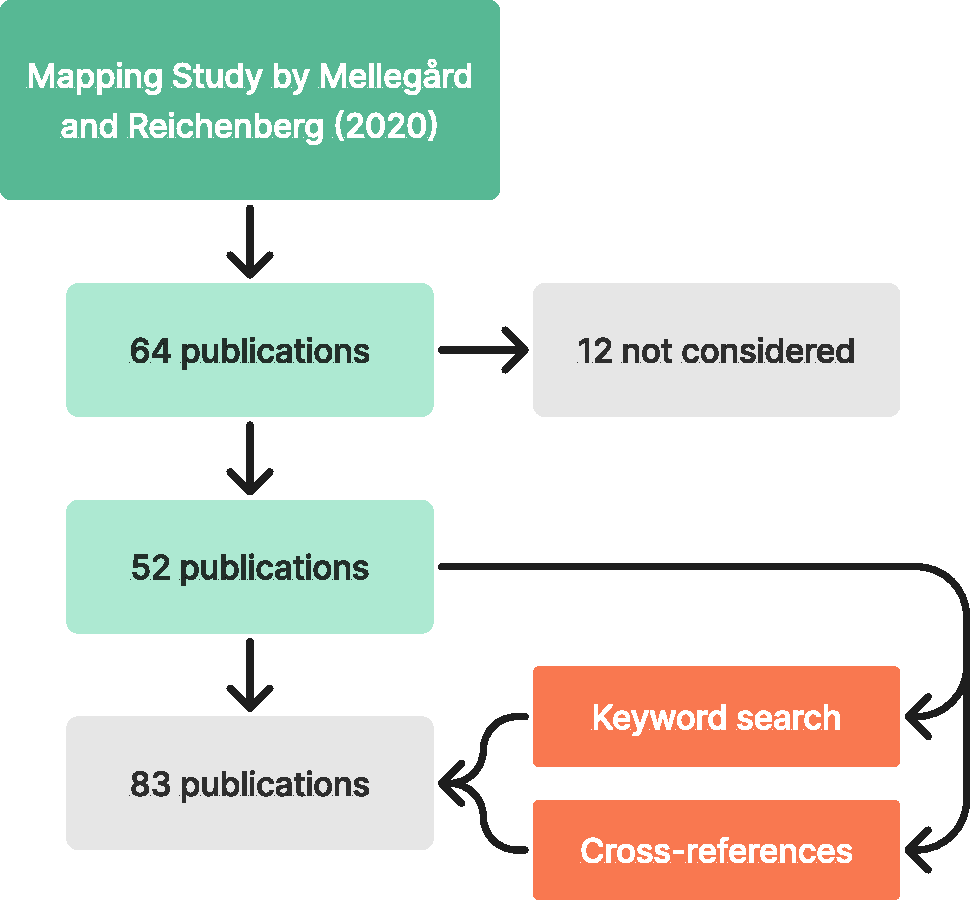
\includegraphics[width=\linewidth]{images/related-work-research-method.pdf} &
  \resizebox{\linewidth}{!}{%% Creator: Matplotlib, PGF backend
%%
%% To include the figure in your LaTeX document, write
%%   \input{<filename>.pgf}
%%
%% Make sure the required packages are loaded in your preamble
%%   \usepackage{pgf}
%%
%% Also ensure that all the required font packages are loaded; for instance,
%% the lmodern package is sometimes necessary when using math font.
%%   \usepackage{lmodern}
%%
%% Figures using additional raster images can only be included by \input if
%% they are in the same directory as the main LaTeX file. For loading figures
%% from other directories you can use the `import` package
%%   \usepackage{import}
%%
%% and then include the figures with
%%   \import{<path to file>}{<filename>.pgf}
%%
%% Matplotlib used the following preamble
%%   \def\mathdefault#1{#1}
%%   \everymath=\expandafter{\the\everymath\displaystyle}
%%   
%%   \makeatletter\@ifpackageloaded{underscore}{}{\usepackage[strings]{underscore}}\makeatother
%%
\begingroup%
\makeatletter%
\begin{pgfpicture}%
\pgfpathrectangle{\pgfpointorigin}{\pgfqpoint{4.490124in}{3.032040in}}%
\pgfusepath{use as bounding box, clip}%
\begin{pgfscope}%
\pgfsetbuttcap%
\pgfsetmiterjoin%
\definecolor{currentfill}{rgb}{1.000000,1.000000,1.000000}%
\pgfsetfillcolor{currentfill}%
\pgfsetlinewidth{0.000000pt}%
\definecolor{currentstroke}{rgb}{1.000000,1.000000,1.000000}%
\pgfsetstrokecolor{currentstroke}%
\pgfsetdash{}{0pt}%
\pgfpathmoveto{\pgfqpoint{0.000000in}{0.000000in}}%
\pgfpathlineto{\pgfqpoint{4.490124in}{0.000000in}}%
\pgfpathlineto{\pgfqpoint{4.490124in}{3.032040in}}%
\pgfpathlineto{\pgfqpoint{0.000000in}{3.032040in}}%
\pgfpathlineto{\pgfqpoint{0.000000in}{0.000000in}}%
\pgfpathclose%
\pgfusepath{fill}%
\end{pgfscope}%
\begin{pgfscope}%
\pgfsetbuttcap%
\pgfsetmiterjoin%
\definecolor{currentfill}{rgb}{1.000000,1.000000,1.000000}%
\pgfsetfillcolor{currentfill}%
\pgfsetlinewidth{0.000000pt}%
\definecolor{currentstroke}{rgb}{0.000000,0.000000,0.000000}%
\pgfsetstrokecolor{currentstroke}%
\pgfsetstrokeopacity{0.000000}%
\pgfsetdash{}{0pt}%
\pgfpathmoveto{\pgfqpoint{0.515124in}{0.622040in}}%
\pgfpathlineto{\pgfqpoint{4.390124in}{0.622040in}}%
\pgfpathlineto{\pgfqpoint{4.390124in}{2.932040in}}%
\pgfpathlineto{\pgfqpoint{0.515124in}{2.932040in}}%
\pgfpathlineto{\pgfqpoint{0.515124in}{0.622040in}}%
\pgfpathclose%
\pgfusepath{fill}%
\end{pgfscope}%
\begin{pgfscope}%
\pgfsetbuttcap%
\pgfsetroundjoin%
\definecolor{currentfill}{rgb}{0.000000,0.000000,0.000000}%
\pgfsetfillcolor{currentfill}%
\pgfsetlinewidth{0.803000pt}%
\definecolor{currentstroke}{rgb}{0.000000,0.000000,0.000000}%
\pgfsetstrokecolor{currentstroke}%
\pgfsetdash{}{0pt}%
\pgfsys@defobject{currentmarker}{\pgfqpoint{0.000000in}{-0.048611in}}{\pgfqpoint{0.000000in}{0.000000in}}{%
\pgfpathmoveto{\pgfqpoint{0.000000in}{0.000000in}}%
\pgfpathlineto{\pgfqpoint{0.000000in}{-0.048611in}}%
\pgfusepath{stroke,fill}%
}%
\begin{pgfscope}%
\pgfsys@transformshift{0.765684in}{0.622040in}%
\pgfsys@useobject{currentmarker}{}%
\end{pgfscope}%
\end{pgfscope}%
\begin{pgfscope}%
\definecolor{textcolor}{rgb}{0.000000,0.000000,0.000000}%
\pgfsetstrokecolor{textcolor}%
\pgfsetfillcolor{textcolor}%
\pgftext[x=0.662763in, y=0.302400in, left, base,rotate=30.000000]{\color{textcolor}{\sffamily\fontsize{10.000000}{12.000000}\selectfont\catcode`\^=\active\def^{\ifmmode\sp\else\^{}\fi}\catcode`\%=\active\def%{\%}$\mathdefault{2006}$}}%
\end{pgfscope}%
\begin{pgfscope}%
\pgfsetbuttcap%
\pgfsetroundjoin%
\definecolor{currentfill}{rgb}{0.000000,0.000000,0.000000}%
\pgfsetfillcolor{currentfill}%
\pgfsetlinewidth{0.803000pt}%
\definecolor{currentstroke}{rgb}{0.000000,0.000000,0.000000}%
\pgfsetstrokecolor{currentstroke}%
\pgfsetdash{}{0pt}%
\pgfsys@defobject{currentmarker}{\pgfqpoint{0.000000in}{-0.048611in}}{\pgfqpoint{0.000000in}{0.000000in}}{%
\pgfpathmoveto{\pgfqpoint{0.000000in}{0.000000in}}%
\pgfpathlineto{\pgfqpoint{0.000000in}{-0.048611in}}%
\pgfusepath{stroke,fill}%
}%
\begin{pgfscope}%
\pgfsys@transformshift{1.162611in}{0.622040in}%
\pgfsys@useobject{currentmarker}{}%
\end{pgfscope}%
\end{pgfscope}%
\begin{pgfscope}%
\definecolor{textcolor}{rgb}{0.000000,0.000000,0.000000}%
\pgfsetstrokecolor{textcolor}%
\pgfsetfillcolor{textcolor}%
\pgftext[x=1.059690in, y=0.302400in, left, base,rotate=30.000000]{\color{textcolor}{\sffamily\fontsize{10.000000}{12.000000}\selectfont\catcode`\^=\active\def^{\ifmmode\sp\else\^{}\fi}\catcode`\%=\active\def%{\%}$\mathdefault{2008}$}}%
\end{pgfscope}%
\begin{pgfscope}%
\pgfsetbuttcap%
\pgfsetroundjoin%
\definecolor{currentfill}{rgb}{0.000000,0.000000,0.000000}%
\pgfsetfillcolor{currentfill}%
\pgfsetlinewidth{0.803000pt}%
\definecolor{currentstroke}{rgb}{0.000000,0.000000,0.000000}%
\pgfsetstrokecolor{currentstroke}%
\pgfsetdash{}{0pt}%
\pgfsys@defobject{currentmarker}{\pgfqpoint{0.000000in}{-0.048611in}}{\pgfqpoint{0.000000in}{0.000000in}}{%
\pgfpathmoveto{\pgfqpoint{0.000000in}{0.000000in}}%
\pgfpathlineto{\pgfqpoint{0.000000in}{-0.048611in}}%
\pgfusepath{stroke,fill}%
}%
\begin{pgfscope}%
\pgfsys@transformshift{1.559538in}{0.622040in}%
\pgfsys@useobject{currentmarker}{}%
\end{pgfscope}%
\end{pgfscope}%
\begin{pgfscope}%
\definecolor{textcolor}{rgb}{0.000000,0.000000,0.000000}%
\pgfsetstrokecolor{textcolor}%
\pgfsetfillcolor{textcolor}%
\pgftext[x=1.456617in, y=0.302400in, left, base,rotate=30.000000]{\color{textcolor}{\sffamily\fontsize{10.000000}{12.000000}\selectfont\catcode`\^=\active\def^{\ifmmode\sp\else\^{}\fi}\catcode`\%=\active\def%{\%}$\mathdefault{2010}$}}%
\end{pgfscope}%
\begin{pgfscope}%
\pgfsetbuttcap%
\pgfsetroundjoin%
\definecolor{currentfill}{rgb}{0.000000,0.000000,0.000000}%
\pgfsetfillcolor{currentfill}%
\pgfsetlinewidth{0.803000pt}%
\definecolor{currentstroke}{rgb}{0.000000,0.000000,0.000000}%
\pgfsetstrokecolor{currentstroke}%
\pgfsetdash{}{0pt}%
\pgfsys@defobject{currentmarker}{\pgfqpoint{0.000000in}{-0.048611in}}{\pgfqpoint{0.000000in}{0.000000in}}{%
\pgfpathmoveto{\pgfqpoint{0.000000in}{0.000000in}}%
\pgfpathlineto{\pgfqpoint{0.000000in}{-0.048611in}}%
\pgfusepath{stroke,fill}%
}%
\begin{pgfscope}%
\pgfsys@transformshift{1.956465in}{0.622040in}%
\pgfsys@useobject{currentmarker}{}%
\end{pgfscope}%
\end{pgfscope}%
\begin{pgfscope}%
\definecolor{textcolor}{rgb}{0.000000,0.000000,0.000000}%
\pgfsetstrokecolor{textcolor}%
\pgfsetfillcolor{textcolor}%
\pgftext[x=1.853544in, y=0.302400in, left, base,rotate=30.000000]{\color{textcolor}{\sffamily\fontsize{10.000000}{12.000000}\selectfont\catcode`\^=\active\def^{\ifmmode\sp\else\^{}\fi}\catcode`\%=\active\def%{\%}$\mathdefault{2012}$}}%
\end{pgfscope}%
\begin{pgfscope}%
\pgfsetbuttcap%
\pgfsetroundjoin%
\definecolor{currentfill}{rgb}{0.000000,0.000000,0.000000}%
\pgfsetfillcolor{currentfill}%
\pgfsetlinewidth{0.803000pt}%
\definecolor{currentstroke}{rgb}{0.000000,0.000000,0.000000}%
\pgfsetstrokecolor{currentstroke}%
\pgfsetdash{}{0pt}%
\pgfsys@defobject{currentmarker}{\pgfqpoint{0.000000in}{-0.048611in}}{\pgfqpoint{0.000000in}{0.000000in}}{%
\pgfpathmoveto{\pgfqpoint{0.000000in}{0.000000in}}%
\pgfpathlineto{\pgfqpoint{0.000000in}{-0.048611in}}%
\pgfusepath{stroke,fill}%
}%
\begin{pgfscope}%
\pgfsys@transformshift{2.353392in}{0.622040in}%
\pgfsys@useobject{currentmarker}{}%
\end{pgfscope}%
\end{pgfscope}%
\begin{pgfscope}%
\definecolor{textcolor}{rgb}{0.000000,0.000000,0.000000}%
\pgfsetstrokecolor{textcolor}%
\pgfsetfillcolor{textcolor}%
\pgftext[x=2.250471in, y=0.302400in, left, base,rotate=30.000000]{\color{textcolor}{\sffamily\fontsize{10.000000}{12.000000}\selectfont\catcode`\^=\active\def^{\ifmmode\sp\else\^{}\fi}\catcode`\%=\active\def%{\%}$\mathdefault{2014}$}}%
\end{pgfscope}%
\begin{pgfscope}%
\pgfsetbuttcap%
\pgfsetroundjoin%
\definecolor{currentfill}{rgb}{0.000000,0.000000,0.000000}%
\pgfsetfillcolor{currentfill}%
\pgfsetlinewidth{0.803000pt}%
\definecolor{currentstroke}{rgb}{0.000000,0.000000,0.000000}%
\pgfsetstrokecolor{currentstroke}%
\pgfsetdash{}{0pt}%
\pgfsys@defobject{currentmarker}{\pgfqpoint{0.000000in}{-0.048611in}}{\pgfqpoint{0.000000in}{0.000000in}}{%
\pgfpathmoveto{\pgfqpoint{0.000000in}{0.000000in}}%
\pgfpathlineto{\pgfqpoint{0.000000in}{-0.048611in}}%
\pgfusepath{stroke,fill}%
}%
\begin{pgfscope}%
\pgfsys@transformshift{2.750319in}{0.622040in}%
\pgfsys@useobject{currentmarker}{}%
\end{pgfscope}%
\end{pgfscope}%
\begin{pgfscope}%
\definecolor{textcolor}{rgb}{0.000000,0.000000,0.000000}%
\pgfsetstrokecolor{textcolor}%
\pgfsetfillcolor{textcolor}%
\pgftext[x=2.647398in, y=0.302400in, left, base,rotate=30.000000]{\color{textcolor}{\sffamily\fontsize{10.000000}{12.000000}\selectfont\catcode`\^=\active\def^{\ifmmode\sp\else\^{}\fi}\catcode`\%=\active\def%{\%}$\mathdefault{2016}$}}%
\end{pgfscope}%
\begin{pgfscope}%
\pgfsetbuttcap%
\pgfsetroundjoin%
\definecolor{currentfill}{rgb}{0.000000,0.000000,0.000000}%
\pgfsetfillcolor{currentfill}%
\pgfsetlinewidth{0.803000pt}%
\definecolor{currentstroke}{rgb}{0.000000,0.000000,0.000000}%
\pgfsetstrokecolor{currentstroke}%
\pgfsetdash{}{0pt}%
\pgfsys@defobject{currentmarker}{\pgfqpoint{0.000000in}{-0.048611in}}{\pgfqpoint{0.000000in}{0.000000in}}{%
\pgfpathmoveto{\pgfqpoint{0.000000in}{0.000000in}}%
\pgfpathlineto{\pgfqpoint{0.000000in}{-0.048611in}}%
\pgfusepath{stroke,fill}%
}%
\begin{pgfscope}%
\pgfsys@transformshift{3.147246in}{0.622040in}%
\pgfsys@useobject{currentmarker}{}%
\end{pgfscope}%
\end{pgfscope}%
\begin{pgfscope}%
\definecolor{textcolor}{rgb}{0.000000,0.000000,0.000000}%
\pgfsetstrokecolor{textcolor}%
\pgfsetfillcolor{textcolor}%
\pgftext[x=3.044325in, y=0.302400in, left, base,rotate=30.000000]{\color{textcolor}{\sffamily\fontsize{10.000000}{12.000000}\selectfont\catcode`\^=\active\def^{\ifmmode\sp\else\^{}\fi}\catcode`\%=\active\def%{\%}$\mathdefault{2018}$}}%
\end{pgfscope}%
\begin{pgfscope}%
\pgfsetbuttcap%
\pgfsetroundjoin%
\definecolor{currentfill}{rgb}{0.000000,0.000000,0.000000}%
\pgfsetfillcolor{currentfill}%
\pgfsetlinewidth{0.803000pt}%
\definecolor{currentstroke}{rgb}{0.000000,0.000000,0.000000}%
\pgfsetstrokecolor{currentstroke}%
\pgfsetdash{}{0pt}%
\pgfsys@defobject{currentmarker}{\pgfqpoint{0.000000in}{-0.048611in}}{\pgfqpoint{0.000000in}{0.000000in}}{%
\pgfpathmoveto{\pgfqpoint{0.000000in}{0.000000in}}%
\pgfpathlineto{\pgfqpoint{0.000000in}{-0.048611in}}%
\pgfusepath{stroke,fill}%
}%
\begin{pgfscope}%
\pgfsys@transformshift{3.544173in}{0.622040in}%
\pgfsys@useobject{currentmarker}{}%
\end{pgfscope}%
\end{pgfscope}%
\begin{pgfscope}%
\definecolor{textcolor}{rgb}{0.000000,0.000000,0.000000}%
\pgfsetstrokecolor{textcolor}%
\pgfsetfillcolor{textcolor}%
\pgftext[x=3.441252in, y=0.302400in, left, base,rotate=30.000000]{\color{textcolor}{\sffamily\fontsize{10.000000}{12.000000}\selectfont\catcode`\^=\active\def^{\ifmmode\sp\else\^{}\fi}\catcode`\%=\active\def%{\%}$\mathdefault{2020}$}}%
\end{pgfscope}%
\begin{pgfscope}%
\pgfsetbuttcap%
\pgfsetroundjoin%
\definecolor{currentfill}{rgb}{0.000000,0.000000,0.000000}%
\pgfsetfillcolor{currentfill}%
\pgfsetlinewidth{0.803000pt}%
\definecolor{currentstroke}{rgb}{0.000000,0.000000,0.000000}%
\pgfsetstrokecolor{currentstroke}%
\pgfsetdash{}{0pt}%
\pgfsys@defobject{currentmarker}{\pgfqpoint{0.000000in}{-0.048611in}}{\pgfqpoint{0.000000in}{0.000000in}}{%
\pgfpathmoveto{\pgfqpoint{0.000000in}{0.000000in}}%
\pgfpathlineto{\pgfqpoint{0.000000in}{-0.048611in}}%
\pgfusepath{stroke,fill}%
}%
\begin{pgfscope}%
\pgfsys@transformshift{3.941100in}{0.622040in}%
\pgfsys@useobject{currentmarker}{}%
\end{pgfscope}%
\end{pgfscope}%
\begin{pgfscope}%
\definecolor{textcolor}{rgb}{0.000000,0.000000,0.000000}%
\pgfsetstrokecolor{textcolor}%
\pgfsetfillcolor{textcolor}%
\pgftext[x=3.838180in, y=0.302400in, left, base,rotate=30.000000]{\color{textcolor}{\sffamily\fontsize{10.000000}{12.000000}\selectfont\catcode`\^=\active\def^{\ifmmode\sp\else\^{}\fi}\catcode`\%=\active\def%{\%}$\mathdefault{2022}$}}%
\end{pgfscope}%
\begin{pgfscope}%
\definecolor{textcolor}{rgb}{0.000000,0.000000,0.000000}%
\pgfsetstrokecolor{textcolor}%
\pgfsetfillcolor{textcolor}%
\pgftext[x=2.452624in,y=0.223457in,,top]{\color{textcolor}{\sffamily\fontsize{10.000000}{12.000000}\selectfont\catcode`\^=\active\def^{\ifmmode\sp\else\^{}\fi}\catcode`\%=\active\def%{\%}Year}}%
\end{pgfscope}%
\begin{pgfscope}%
\pgfpathrectangle{\pgfqpoint{0.515124in}{0.622040in}}{\pgfqpoint{3.875000in}{2.310000in}}%
\pgfusepath{clip}%
\pgfsetbuttcap%
\pgfsetroundjoin%
\pgfsetlinewidth{0.501875pt}%
\definecolor{currentstroke}{rgb}{0.690196,0.690196,0.690196}%
\pgfsetstrokecolor{currentstroke}%
\pgfsetstrokeopacity{0.500000}%
\pgfsetdash{{1.850000pt}{0.800000pt}}{0.000000pt}%
\pgfpathmoveto{\pgfqpoint{0.515124in}{0.622040in}}%
\pgfpathlineto{\pgfqpoint{4.390124in}{0.622040in}}%
\pgfusepath{stroke}%
\end{pgfscope}%
\begin{pgfscope}%
\pgfsetbuttcap%
\pgfsetroundjoin%
\definecolor{currentfill}{rgb}{0.000000,0.000000,0.000000}%
\pgfsetfillcolor{currentfill}%
\pgfsetlinewidth{0.803000pt}%
\definecolor{currentstroke}{rgb}{0.000000,0.000000,0.000000}%
\pgfsetstrokecolor{currentstroke}%
\pgfsetdash{}{0pt}%
\pgfsys@defobject{currentmarker}{\pgfqpoint{-0.048611in}{0.000000in}}{\pgfqpoint{-0.000000in}{0.000000in}}{%
\pgfpathmoveto{\pgfqpoint{-0.000000in}{0.000000in}}%
\pgfpathlineto{\pgfqpoint{-0.048611in}{0.000000in}}%
\pgfusepath{stroke,fill}%
}%
\begin{pgfscope}%
\pgfsys@transformshift{0.515124in}{0.622040in}%
\pgfsys@useobject{currentmarker}{}%
\end{pgfscope}%
\end{pgfscope}%
\begin{pgfscope}%
\definecolor{textcolor}{rgb}{0.000000,0.000000,0.000000}%
\pgfsetstrokecolor{textcolor}%
\pgfsetfillcolor{textcolor}%
\pgftext[x=0.348457in, y=0.573815in, left, base]{\color{textcolor}{\sffamily\fontsize{10.000000}{12.000000}\selectfont\catcode`\^=\active\def^{\ifmmode\sp\else\^{}\fi}\catcode`\%=\active\def%{\%}$\mathdefault{0}$}}%
\end{pgfscope}%
\begin{pgfscope}%
\pgfpathrectangle{\pgfqpoint{0.515124in}{0.622040in}}{\pgfqpoint{3.875000in}{2.310000in}}%
\pgfusepath{clip}%
\pgfsetbuttcap%
\pgfsetroundjoin%
\pgfsetlinewidth{0.501875pt}%
\definecolor{currentstroke}{rgb}{0.690196,0.690196,0.690196}%
\pgfsetstrokecolor{currentstroke}%
\pgfsetstrokeopacity{0.500000}%
\pgfsetdash{{1.850000pt}{0.800000pt}}{0.000000pt}%
\pgfpathmoveto{\pgfqpoint{0.515124in}{1.042040in}}%
\pgfpathlineto{\pgfqpoint{4.390124in}{1.042040in}}%
\pgfusepath{stroke}%
\end{pgfscope}%
\begin{pgfscope}%
\pgfsetbuttcap%
\pgfsetroundjoin%
\definecolor{currentfill}{rgb}{0.000000,0.000000,0.000000}%
\pgfsetfillcolor{currentfill}%
\pgfsetlinewidth{0.803000pt}%
\definecolor{currentstroke}{rgb}{0.000000,0.000000,0.000000}%
\pgfsetstrokecolor{currentstroke}%
\pgfsetdash{}{0pt}%
\pgfsys@defobject{currentmarker}{\pgfqpoint{-0.048611in}{0.000000in}}{\pgfqpoint{-0.000000in}{0.000000in}}{%
\pgfpathmoveto{\pgfqpoint{-0.000000in}{0.000000in}}%
\pgfpathlineto{\pgfqpoint{-0.048611in}{0.000000in}}%
\pgfusepath{stroke,fill}%
}%
\begin{pgfscope}%
\pgfsys@transformshift{0.515124in}{1.042040in}%
\pgfsys@useobject{currentmarker}{}%
\end{pgfscope}%
\end{pgfscope}%
\begin{pgfscope}%
\definecolor{textcolor}{rgb}{0.000000,0.000000,0.000000}%
\pgfsetstrokecolor{textcolor}%
\pgfsetfillcolor{textcolor}%
\pgftext[x=0.348457in, y=0.993815in, left, base]{\color{textcolor}{\sffamily\fontsize{10.000000}{12.000000}\selectfont\catcode`\^=\active\def^{\ifmmode\sp\else\^{}\fi}\catcode`\%=\active\def%{\%}$\mathdefault{2}$}}%
\end{pgfscope}%
\begin{pgfscope}%
\pgfpathrectangle{\pgfqpoint{0.515124in}{0.622040in}}{\pgfqpoint{3.875000in}{2.310000in}}%
\pgfusepath{clip}%
\pgfsetbuttcap%
\pgfsetroundjoin%
\pgfsetlinewidth{0.501875pt}%
\definecolor{currentstroke}{rgb}{0.690196,0.690196,0.690196}%
\pgfsetstrokecolor{currentstroke}%
\pgfsetstrokeopacity{0.500000}%
\pgfsetdash{{1.850000pt}{0.800000pt}}{0.000000pt}%
\pgfpathmoveto{\pgfqpoint{0.515124in}{1.462040in}}%
\pgfpathlineto{\pgfqpoint{4.390124in}{1.462040in}}%
\pgfusepath{stroke}%
\end{pgfscope}%
\begin{pgfscope}%
\pgfsetbuttcap%
\pgfsetroundjoin%
\definecolor{currentfill}{rgb}{0.000000,0.000000,0.000000}%
\pgfsetfillcolor{currentfill}%
\pgfsetlinewidth{0.803000pt}%
\definecolor{currentstroke}{rgb}{0.000000,0.000000,0.000000}%
\pgfsetstrokecolor{currentstroke}%
\pgfsetdash{}{0pt}%
\pgfsys@defobject{currentmarker}{\pgfqpoint{-0.048611in}{0.000000in}}{\pgfqpoint{-0.000000in}{0.000000in}}{%
\pgfpathmoveto{\pgfqpoint{-0.000000in}{0.000000in}}%
\pgfpathlineto{\pgfqpoint{-0.048611in}{0.000000in}}%
\pgfusepath{stroke,fill}%
}%
\begin{pgfscope}%
\pgfsys@transformshift{0.515124in}{1.462040in}%
\pgfsys@useobject{currentmarker}{}%
\end{pgfscope}%
\end{pgfscope}%
\begin{pgfscope}%
\definecolor{textcolor}{rgb}{0.000000,0.000000,0.000000}%
\pgfsetstrokecolor{textcolor}%
\pgfsetfillcolor{textcolor}%
\pgftext[x=0.348457in, y=1.413815in, left, base]{\color{textcolor}{\sffamily\fontsize{10.000000}{12.000000}\selectfont\catcode`\^=\active\def^{\ifmmode\sp\else\^{}\fi}\catcode`\%=\active\def%{\%}$\mathdefault{4}$}}%
\end{pgfscope}%
\begin{pgfscope}%
\pgfpathrectangle{\pgfqpoint{0.515124in}{0.622040in}}{\pgfqpoint{3.875000in}{2.310000in}}%
\pgfusepath{clip}%
\pgfsetbuttcap%
\pgfsetroundjoin%
\pgfsetlinewidth{0.501875pt}%
\definecolor{currentstroke}{rgb}{0.690196,0.690196,0.690196}%
\pgfsetstrokecolor{currentstroke}%
\pgfsetstrokeopacity{0.500000}%
\pgfsetdash{{1.850000pt}{0.800000pt}}{0.000000pt}%
\pgfpathmoveto{\pgfqpoint{0.515124in}{1.882040in}}%
\pgfpathlineto{\pgfqpoint{4.390124in}{1.882040in}}%
\pgfusepath{stroke}%
\end{pgfscope}%
\begin{pgfscope}%
\pgfsetbuttcap%
\pgfsetroundjoin%
\definecolor{currentfill}{rgb}{0.000000,0.000000,0.000000}%
\pgfsetfillcolor{currentfill}%
\pgfsetlinewidth{0.803000pt}%
\definecolor{currentstroke}{rgb}{0.000000,0.000000,0.000000}%
\pgfsetstrokecolor{currentstroke}%
\pgfsetdash{}{0pt}%
\pgfsys@defobject{currentmarker}{\pgfqpoint{-0.048611in}{0.000000in}}{\pgfqpoint{-0.000000in}{0.000000in}}{%
\pgfpathmoveto{\pgfqpoint{-0.000000in}{0.000000in}}%
\pgfpathlineto{\pgfqpoint{-0.048611in}{0.000000in}}%
\pgfusepath{stroke,fill}%
}%
\begin{pgfscope}%
\pgfsys@transformshift{0.515124in}{1.882040in}%
\pgfsys@useobject{currentmarker}{}%
\end{pgfscope}%
\end{pgfscope}%
\begin{pgfscope}%
\definecolor{textcolor}{rgb}{0.000000,0.000000,0.000000}%
\pgfsetstrokecolor{textcolor}%
\pgfsetfillcolor{textcolor}%
\pgftext[x=0.348457in, y=1.833815in, left, base]{\color{textcolor}{\sffamily\fontsize{10.000000}{12.000000}\selectfont\catcode`\^=\active\def^{\ifmmode\sp\else\^{}\fi}\catcode`\%=\active\def%{\%}$\mathdefault{6}$}}%
\end{pgfscope}%
\begin{pgfscope}%
\pgfpathrectangle{\pgfqpoint{0.515124in}{0.622040in}}{\pgfqpoint{3.875000in}{2.310000in}}%
\pgfusepath{clip}%
\pgfsetbuttcap%
\pgfsetroundjoin%
\pgfsetlinewidth{0.501875pt}%
\definecolor{currentstroke}{rgb}{0.690196,0.690196,0.690196}%
\pgfsetstrokecolor{currentstroke}%
\pgfsetstrokeopacity{0.500000}%
\pgfsetdash{{1.850000pt}{0.800000pt}}{0.000000pt}%
\pgfpathmoveto{\pgfqpoint{0.515124in}{2.302040in}}%
\pgfpathlineto{\pgfqpoint{4.390124in}{2.302040in}}%
\pgfusepath{stroke}%
\end{pgfscope}%
\begin{pgfscope}%
\pgfsetbuttcap%
\pgfsetroundjoin%
\definecolor{currentfill}{rgb}{0.000000,0.000000,0.000000}%
\pgfsetfillcolor{currentfill}%
\pgfsetlinewidth{0.803000pt}%
\definecolor{currentstroke}{rgb}{0.000000,0.000000,0.000000}%
\pgfsetstrokecolor{currentstroke}%
\pgfsetdash{}{0pt}%
\pgfsys@defobject{currentmarker}{\pgfqpoint{-0.048611in}{0.000000in}}{\pgfqpoint{-0.000000in}{0.000000in}}{%
\pgfpathmoveto{\pgfqpoint{-0.000000in}{0.000000in}}%
\pgfpathlineto{\pgfqpoint{-0.048611in}{0.000000in}}%
\pgfusepath{stroke,fill}%
}%
\begin{pgfscope}%
\pgfsys@transformshift{0.515124in}{2.302040in}%
\pgfsys@useobject{currentmarker}{}%
\end{pgfscope}%
\end{pgfscope}%
\begin{pgfscope}%
\definecolor{textcolor}{rgb}{0.000000,0.000000,0.000000}%
\pgfsetstrokecolor{textcolor}%
\pgfsetfillcolor{textcolor}%
\pgftext[x=0.348457in, y=2.253815in, left, base]{\color{textcolor}{\sffamily\fontsize{10.000000}{12.000000}\selectfont\catcode`\^=\active\def^{\ifmmode\sp\else\^{}\fi}\catcode`\%=\active\def%{\%}$\mathdefault{8}$}}%
\end{pgfscope}%
\begin{pgfscope}%
\pgfpathrectangle{\pgfqpoint{0.515124in}{0.622040in}}{\pgfqpoint{3.875000in}{2.310000in}}%
\pgfusepath{clip}%
\pgfsetbuttcap%
\pgfsetroundjoin%
\pgfsetlinewidth{0.501875pt}%
\definecolor{currentstroke}{rgb}{0.690196,0.690196,0.690196}%
\pgfsetstrokecolor{currentstroke}%
\pgfsetstrokeopacity{0.500000}%
\pgfsetdash{{1.850000pt}{0.800000pt}}{0.000000pt}%
\pgfpathmoveto{\pgfqpoint{0.515124in}{2.722040in}}%
\pgfpathlineto{\pgfqpoint{4.390124in}{2.722040in}}%
\pgfusepath{stroke}%
\end{pgfscope}%
\begin{pgfscope}%
\pgfsetbuttcap%
\pgfsetroundjoin%
\definecolor{currentfill}{rgb}{0.000000,0.000000,0.000000}%
\pgfsetfillcolor{currentfill}%
\pgfsetlinewidth{0.803000pt}%
\definecolor{currentstroke}{rgb}{0.000000,0.000000,0.000000}%
\pgfsetstrokecolor{currentstroke}%
\pgfsetdash{}{0pt}%
\pgfsys@defobject{currentmarker}{\pgfqpoint{-0.048611in}{0.000000in}}{\pgfqpoint{-0.000000in}{0.000000in}}{%
\pgfpathmoveto{\pgfqpoint{-0.000000in}{0.000000in}}%
\pgfpathlineto{\pgfqpoint{-0.048611in}{0.000000in}}%
\pgfusepath{stroke,fill}%
}%
\begin{pgfscope}%
\pgfsys@transformshift{0.515124in}{2.722040in}%
\pgfsys@useobject{currentmarker}{}%
\end{pgfscope}%
\end{pgfscope}%
\begin{pgfscope}%
\definecolor{textcolor}{rgb}{0.000000,0.000000,0.000000}%
\pgfsetstrokecolor{textcolor}%
\pgfsetfillcolor{textcolor}%
\pgftext[x=0.279012in, y=2.673815in, left, base]{\color{textcolor}{\sffamily\fontsize{10.000000}{12.000000}\selectfont\catcode`\^=\active\def^{\ifmmode\sp\else\^{}\fi}\catcode`\%=\active\def%{\%}$\mathdefault{10}$}}%
\end{pgfscope}%
\begin{pgfscope}%
\definecolor{textcolor}{rgb}{0.000000,0.000000,0.000000}%
\pgfsetstrokecolor{textcolor}%
\pgfsetfillcolor{textcolor}%
\pgftext[x=0.223457in,y=1.777040in,,bottom,rotate=90.000000]{\color{textcolor}{\sffamily\fontsize{10.000000}{12.000000}\selectfont\catcode`\^=\active\def^{\ifmmode\sp\else\^{}\fi}\catcode`\%=\active\def%{\%}\# Publications}}%
\end{pgfscope}%
\begin{pgfscope}%
\pgfpathrectangle{\pgfqpoint{0.515124in}{0.622040in}}{\pgfqpoint{3.875000in}{2.310000in}}%
\pgfusepath{clip}%
\pgfsetbuttcap%
\pgfsetmiterjoin%
\definecolor{currentfill}{rgb}{0.000000,0.411765,0.705882}%
\pgfsetfillcolor{currentfill}%
\pgfsetlinewidth{0.000000pt}%
\definecolor{currentstroke}{rgb}{0.000000,0.000000,0.000000}%
\pgfsetstrokecolor{currentstroke}%
\pgfsetstrokeopacity{0.000000}%
\pgfsetdash{}{0pt}%
\pgfpathmoveto{\pgfqpoint{0.691260in}{0.622040in}}%
\pgfpathlineto{\pgfqpoint{0.840108in}{0.622040in}}%
\pgfpathlineto{\pgfqpoint{0.840108in}{0.832040in}}%
\pgfpathlineto{\pgfqpoint{0.691260in}{0.832040in}}%
\pgfpathlineto{\pgfqpoint{0.691260in}{0.622040in}}%
\pgfpathclose%
\pgfusepath{fill}%
\end{pgfscope}%
\begin{pgfscope}%
\pgfpathrectangle{\pgfqpoint{0.515124in}{0.622040in}}{\pgfqpoint{3.875000in}{2.310000in}}%
\pgfusepath{clip}%
\pgfsetbuttcap%
\pgfsetmiterjoin%
\definecolor{currentfill}{rgb}{0.000000,0.411765,0.705882}%
\pgfsetfillcolor{currentfill}%
\pgfsetlinewidth{0.000000pt}%
\definecolor{currentstroke}{rgb}{0.000000,0.000000,0.000000}%
\pgfsetstrokecolor{currentstroke}%
\pgfsetstrokeopacity{0.000000}%
\pgfsetdash{}{0pt}%
\pgfpathmoveto{\pgfqpoint{0.889724in}{0.622040in}}%
\pgfpathlineto{\pgfqpoint{1.038571in}{0.622040in}}%
\pgfpathlineto{\pgfqpoint{1.038571in}{0.622040in}}%
\pgfpathlineto{\pgfqpoint{0.889724in}{0.622040in}}%
\pgfpathlineto{\pgfqpoint{0.889724in}{0.622040in}}%
\pgfpathclose%
\pgfusepath{fill}%
\end{pgfscope}%
\begin{pgfscope}%
\pgfpathrectangle{\pgfqpoint{0.515124in}{0.622040in}}{\pgfqpoint{3.875000in}{2.310000in}}%
\pgfusepath{clip}%
\pgfsetbuttcap%
\pgfsetmiterjoin%
\definecolor{currentfill}{rgb}{0.000000,0.411765,0.705882}%
\pgfsetfillcolor{currentfill}%
\pgfsetlinewidth{0.000000pt}%
\definecolor{currentstroke}{rgb}{0.000000,0.000000,0.000000}%
\pgfsetstrokecolor{currentstroke}%
\pgfsetstrokeopacity{0.000000}%
\pgfsetdash{}{0pt}%
\pgfpathmoveto{\pgfqpoint{1.088187in}{0.622040in}}%
\pgfpathlineto{\pgfqpoint{1.237035in}{0.622040in}}%
\pgfpathlineto{\pgfqpoint{1.237035in}{0.832040in}}%
\pgfpathlineto{\pgfqpoint{1.088187in}{0.832040in}}%
\pgfpathlineto{\pgfqpoint{1.088187in}{0.622040in}}%
\pgfpathclose%
\pgfusepath{fill}%
\end{pgfscope}%
\begin{pgfscope}%
\pgfpathrectangle{\pgfqpoint{0.515124in}{0.622040in}}{\pgfqpoint{3.875000in}{2.310000in}}%
\pgfusepath{clip}%
\pgfsetbuttcap%
\pgfsetmiterjoin%
\definecolor{currentfill}{rgb}{0.000000,0.411765,0.705882}%
\pgfsetfillcolor{currentfill}%
\pgfsetlinewidth{0.000000pt}%
\definecolor{currentstroke}{rgb}{0.000000,0.000000,0.000000}%
\pgfsetstrokecolor{currentstroke}%
\pgfsetstrokeopacity{0.000000}%
\pgfsetdash{}{0pt}%
\pgfpathmoveto{\pgfqpoint{1.286651in}{0.622040in}}%
\pgfpathlineto{\pgfqpoint{1.435498in}{0.622040in}}%
\pgfpathlineto{\pgfqpoint{1.435498in}{0.622040in}}%
\pgfpathlineto{\pgfqpoint{1.286651in}{0.622040in}}%
\pgfpathlineto{\pgfqpoint{1.286651in}{0.622040in}}%
\pgfpathclose%
\pgfusepath{fill}%
\end{pgfscope}%
\begin{pgfscope}%
\pgfpathrectangle{\pgfqpoint{0.515124in}{0.622040in}}{\pgfqpoint{3.875000in}{2.310000in}}%
\pgfusepath{clip}%
\pgfsetbuttcap%
\pgfsetmiterjoin%
\definecolor{currentfill}{rgb}{0.000000,0.411765,0.705882}%
\pgfsetfillcolor{currentfill}%
\pgfsetlinewidth{0.000000pt}%
\definecolor{currentstroke}{rgb}{0.000000,0.000000,0.000000}%
\pgfsetstrokecolor{currentstroke}%
\pgfsetstrokeopacity{0.000000}%
\pgfsetdash{}{0pt}%
\pgfpathmoveto{\pgfqpoint{1.485114in}{0.622040in}}%
\pgfpathlineto{\pgfqpoint{1.633962in}{0.622040in}}%
\pgfpathlineto{\pgfqpoint{1.633962in}{0.832040in}}%
\pgfpathlineto{\pgfqpoint{1.485114in}{0.832040in}}%
\pgfpathlineto{\pgfqpoint{1.485114in}{0.622040in}}%
\pgfpathclose%
\pgfusepath{fill}%
\end{pgfscope}%
\begin{pgfscope}%
\pgfpathrectangle{\pgfqpoint{0.515124in}{0.622040in}}{\pgfqpoint{3.875000in}{2.310000in}}%
\pgfusepath{clip}%
\pgfsetbuttcap%
\pgfsetmiterjoin%
\definecolor{currentfill}{rgb}{0.000000,0.411765,0.705882}%
\pgfsetfillcolor{currentfill}%
\pgfsetlinewidth{0.000000pt}%
\definecolor{currentstroke}{rgb}{0.000000,0.000000,0.000000}%
\pgfsetstrokecolor{currentstroke}%
\pgfsetstrokeopacity{0.000000}%
\pgfsetdash{}{0pt}%
\pgfpathmoveto{\pgfqpoint{1.683578in}{0.622040in}}%
\pgfpathlineto{\pgfqpoint{1.832425in}{0.622040in}}%
\pgfpathlineto{\pgfqpoint{1.832425in}{2.092040in}}%
\pgfpathlineto{\pgfqpoint{1.683578in}{2.092040in}}%
\pgfpathlineto{\pgfqpoint{1.683578in}{0.622040in}}%
\pgfpathclose%
\pgfusepath{fill}%
\end{pgfscope}%
\begin{pgfscope}%
\pgfpathrectangle{\pgfqpoint{0.515124in}{0.622040in}}{\pgfqpoint{3.875000in}{2.310000in}}%
\pgfusepath{clip}%
\pgfsetbuttcap%
\pgfsetmiterjoin%
\definecolor{currentfill}{rgb}{0.000000,0.411765,0.705882}%
\pgfsetfillcolor{currentfill}%
\pgfsetlinewidth{0.000000pt}%
\definecolor{currentstroke}{rgb}{0.000000,0.000000,0.000000}%
\pgfsetstrokecolor{currentstroke}%
\pgfsetstrokeopacity{0.000000}%
\pgfsetdash{}{0pt}%
\pgfpathmoveto{\pgfqpoint{1.882041in}{0.622040in}}%
\pgfpathlineto{\pgfqpoint{2.030889in}{0.622040in}}%
\pgfpathlineto{\pgfqpoint{2.030889in}{1.882040in}}%
\pgfpathlineto{\pgfqpoint{1.882041in}{1.882040in}}%
\pgfpathlineto{\pgfqpoint{1.882041in}{0.622040in}}%
\pgfpathclose%
\pgfusepath{fill}%
\end{pgfscope}%
\begin{pgfscope}%
\pgfpathrectangle{\pgfqpoint{0.515124in}{0.622040in}}{\pgfqpoint{3.875000in}{2.310000in}}%
\pgfusepath{clip}%
\pgfsetbuttcap%
\pgfsetmiterjoin%
\definecolor{currentfill}{rgb}{0.000000,0.411765,0.705882}%
\pgfsetfillcolor{currentfill}%
\pgfsetlinewidth{0.000000pt}%
\definecolor{currentstroke}{rgb}{0.000000,0.000000,0.000000}%
\pgfsetstrokecolor{currentstroke}%
\pgfsetstrokeopacity{0.000000}%
\pgfsetdash{}{0pt}%
\pgfpathmoveto{\pgfqpoint{2.080505in}{0.622040in}}%
\pgfpathlineto{\pgfqpoint{2.229352in}{0.622040in}}%
\pgfpathlineto{\pgfqpoint{2.229352in}{2.092040in}}%
\pgfpathlineto{\pgfqpoint{2.080505in}{2.092040in}}%
\pgfpathlineto{\pgfqpoint{2.080505in}{0.622040in}}%
\pgfpathclose%
\pgfusepath{fill}%
\end{pgfscope}%
\begin{pgfscope}%
\pgfpathrectangle{\pgfqpoint{0.515124in}{0.622040in}}{\pgfqpoint{3.875000in}{2.310000in}}%
\pgfusepath{clip}%
\pgfsetbuttcap%
\pgfsetmiterjoin%
\definecolor{currentfill}{rgb}{0.000000,0.411765,0.705882}%
\pgfsetfillcolor{currentfill}%
\pgfsetlinewidth{0.000000pt}%
\definecolor{currentstroke}{rgb}{0.000000,0.000000,0.000000}%
\pgfsetstrokecolor{currentstroke}%
\pgfsetstrokeopacity{0.000000}%
\pgfsetdash{}{0pt}%
\pgfpathmoveto{\pgfqpoint{2.278968in}{0.622040in}}%
\pgfpathlineto{\pgfqpoint{2.427816in}{0.622040in}}%
\pgfpathlineto{\pgfqpoint{2.427816in}{2.092040in}}%
\pgfpathlineto{\pgfqpoint{2.278968in}{2.092040in}}%
\pgfpathlineto{\pgfqpoint{2.278968in}{0.622040in}}%
\pgfpathclose%
\pgfusepath{fill}%
\end{pgfscope}%
\begin{pgfscope}%
\pgfpathrectangle{\pgfqpoint{0.515124in}{0.622040in}}{\pgfqpoint{3.875000in}{2.310000in}}%
\pgfusepath{clip}%
\pgfsetbuttcap%
\pgfsetmiterjoin%
\definecolor{currentfill}{rgb}{0.000000,0.411765,0.705882}%
\pgfsetfillcolor{currentfill}%
\pgfsetlinewidth{0.000000pt}%
\definecolor{currentstroke}{rgb}{0.000000,0.000000,0.000000}%
\pgfsetstrokecolor{currentstroke}%
\pgfsetstrokeopacity{0.000000}%
\pgfsetdash{}{0pt}%
\pgfpathmoveto{\pgfqpoint{2.477432in}{0.622040in}}%
\pgfpathlineto{\pgfqpoint{2.626279in}{0.622040in}}%
\pgfpathlineto{\pgfqpoint{2.626279in}{1.252040in}}%
\pgfpathlineto{\pgfqpoint{2.477432in}{1.252040in}}%
\pgfpathlineto{\pgfqpoint{2.477432in}{0.622040in}}%
\pgfpathclose%
\pgfusepath{fill}%
\end{pgfscope}%
\begin{pgfscope}%
\pgfpathrectangle{\pgfqpoint{0.515124in}{0.622040in}}{\pgfqpoint{3.875000in}{2.310000in}}%
\pgfusepath{clip}%
\pgfsetbuttcap%
\pgfsetmiterjoin%
\definecolor{currentfill}{rgb}{0.000000,0.411765,0.705882}%
\pgfsetfillcolor{currentfill}%
\pgfsetlinewidth{0.000000pt}%
\definecolor{currentstroke}{rgb}{0.000000,0.000000,0.000000}%
\pgfsetstrokecolor{currentstroke}%
\pgfsetstrokeopacity{0.000000}%
\pgfsetdash{}{0pt}%
\pgfpathmoveto{\pgfqpoint{2.675895in}{0.622040in}}%
\pgfpathlineto{\pgfqpoint{2.824743in}{0.622040in}}%
\pgfpathlineto{\pgfqpoint{2.824743in}{1.882040in}}%
\pgfpathlineto{\pgfqpoint{2.675895in}{1.882040in}}%
\pgfpathlineto{\pgfqpoint{2.675895in}{0.622040in}}%
\pgfpathclose%
\pgfusepath{fill}%
\end{pgfscope}%
\begin{pgfscope}%
\pgfpathrectangle{\pgfqpoint{0.515124in}{0.622040in}}{\pgfqpoint{3.875000in}{2.310000in}}%
\pgfusepath{clip}%
\pgfsetbuttcap%
\pgfsetmiterjoin%
\definecolor{currentfill}{rgb}{0.000000,0.411765,0.705882}%
\pgfsetfillcolor{currentfill}%
\pgfsetlinewidth{0.000000pt}%
\definecolor{currentstroke}{rgb}{0.000000,0.000000,0.000000}%
\pgfsetstrokecolor{currentstroke}%
\pgfsetstrokeopacity{0.000000}%
\pgfsetdash{}{0pt}%
\pgfpathmoveto{\pgfqpoint{2.874359in}{0.622040in}}%
\pgfpathlineto{\pgfqpoint{3.023206in}{0.622040in}}%
\pgfpathlineto{\pgfqpoint{3.023206in}{1.042040in}}%
\pgfpathlineto{\pgfqpoint{2.874359in}{1.042040in}}%
\pgfpathlineto{\pgfqpoint{2.874359in}{0.622040in}}%
\pgfpathclose%
\pgfusepath{fill}%
\end{pgfscope}%
\begin{pgfscope}%
\pgfpathrectangle{\pgfqpoint{0.515124in}{0.622040in}}{\pgfqpoint{3.875000in}{2.310000in}}%
\pgfusepath{clip}%
\pgfsetbuttcap%
\pgfsetmiterjoin%
\definecolor{currentfill}{rgb}{0.000000,0.411765,0.705882}%
\pgfsetfillcolor{currentfill}%
\pgfsetlinewidth{0.000000pt}%
\definecolor{currentstroke}{rgb}{0.000000,0.000000,0.000000}%
\pgfsetstrokecolor{currentstroke}%
\pgfsetstrokeopacity{0.000000}%
\pgfsetdash{}{0pt}%
\pgfpathmoveto{\pgfqpoint{3.072822in}{0.622040in}}%
\pgfpathlineto{\pgfqpoint{3.221670in}{0.622040in}}%
\pgfpathlineto{\pgfqpoint{3.221670in}{2.302040in}}%
\pgfpathlineto{\pgfqpoint{3.072822in}{2.302040in}}%
\pgfpathlineto{\pgfqpoint{3.072822in}{0.622040in}}%
\pgfpathclose%
\pgfusepath{fill}%
\end{pgfscope}%
\begin{pgfscope}%
\pgfpathrectangle{\pgfqpoint{0.515124in}{0.622040in}}{\pgfqpoint{3.875000in}{2.310000in}}%
\pgfusepath{clip}%
\pgfsetbuttcap%
\pgfsetmiterjoin%
\definecolor{currentfill}{rgb}{0.000000,0.411765,0.705882}%
\pgfsetfillcolor{currentfill}%
\pgfsetlinewidth{0.000000pt}%
\definecolor{currentstroke}{rgb}{0.000000,0.000000,0.000000}%
\pgfsetstrokecolor{currentstroke}%
\pgfsetstrokeopacity{0.000000}%
\pgfsetdash{}{0pt}%
\pgfpathmoveto{\pgfqpoint{3.271286in}{0.622040in}}%
\pgfpathlineto{\pgfqpoint{3.420133in}{0.622040in}}%
\pgfpathlineto{\pgfqpoint{3.420133in}{1.042040in}}%
\pgfpathlineto{\pgfqpoint{3.271286in}{1.042040in}}%
\pgfpathlineto{\pgfqpoint{3.271286in}{0.622040in}}%
\pgfpathclose%
\pgfusepath{fill}%
\end{pgfscope}%
\begin{pgfscope}%
\pgfpathrectangle{\pgfqpoint{0.515124in}{0.622040in}}{\pgfqpoint{3.875000in}{2.310000in}}%
\pgfusepath{clip}%
\pgfsetbuttcap%
\pgfsetmiterjoin%
\definecolor{currentfill}{rgb}{0.000000,0.411765,0.705882}%
\pgfsetfillcolor{currentfill}%
\pgfsetlinewidth{0.000000pt}%
\definecolor{currentstroke}{rgb}{0.000000,0.000000,0.000000}%
\pgfsetstrokecolor{currentstroke}%
\pgfsetstrokeopacity{0.000000}%
\pgfsetdash{}{0pt}%
\pgfpathmoveto{\pgfqpoint{3.469749in}{0.622040in}}%
\pgfpathlineto{\pgfqpoint{3.618597in}{0.622040in}}%
\pgfpathlineto{\pgfqpoint{3.618597in}{0.622040in}}%
\pgfpathlineto{\pgfqpoint{3.469749in}{0.622040in}}%
\pgfpathlineto{\pgfqpoint{3.469749in}{0.622040in}}%
\pgfpathclose%
\pgfusepath{fill}%
\end{pgfscope}%
\begin{pgfscope}%
\pgfpathrectangle{\pgfqpoint{0.515124in}{0.622040in}}{\pgfqpoint{3.875000in}{2.310000in}}%
\pgfusepath{clip}%
\pgfsetbuttcap%
\pgfsetmiterjoin%
\definecolor{currentfill}{rgb}{0.000000,0.411765,0.705882}%
\pgfsetfillcolor{currentfill}%
\pgfsetlinewidth{0.000000pt}%
\definecolor{currentstroke}{rgb}{0.000000,0.000000,0.000000}%
\pgfsetstrokecolor{currentstroke}%
\pgfsetstrokeopacity{0.000000}%
\pgfsetdash{}{0pt}%
\pgfpathmoveto{\pgfqpoint{3.668213in}{0.622040in}}%
\pgfpathlineto{\pgfqpoint{3.817060in}{0.622040in}}%
\pgfpathlineto{\pgfqpoint{3.817060in}{0.622040in}}%
\pgfpathlineto{\pgfqpoint{3.668213in}{0.622040in}}%
\pgfpathlineto{\pgfqpoint{3.668213in}{0.622040in}}%
\pgfpathclose%
\pgfusepath{fill}%
\end{pgfscope}%
\begin{pgfscope}%
\pgfpathrectangle{\pgfqpoint{0.515124in}{0.622040in}}{\pgfqpoint{3.875000in}{2.310000in}}%
\pgfusepath{clip}%
\pgfsetbuttcap%
\pgfsetmiterjoin%
\definecolor{currentfill}{rgb}{0.000000,0.411765,0.705882}%
\pgfsetfillcolor{currentfill}%
\pgfsetlinewidth{0.000000pt}%
\definecolor{currentstroke}{rgb}{0.000000,0.000000,0.000000}%
\pgfsetstrokecolor{currentstroke}%
\pgfsetstrokeopacity{0.000000}%
\pgfsetdash{}{0pt}%
\pgfpathmoveto{\pgfqpoint{3.866676in}{0.622040in}}%
\pgfpathlineto{\pgfqpoint{4.015524in}{0.622040in}}%
\pgfpathlineto{\pgfqpoint{4.015524in}{0.622040in}}%
\pgfpathlineto{\pgfqpoint{3.866676in}{0.622040in}}%
\pgfpathlineto{\pgfqpoint{3.866676in}{0.622040in}}%
\pgfpathclose%
\pgfusepath{fill}%
\end{pgfscope}%
\begin{pgfscope}%
\pgfpathrectangle{\pgfqpoint{0.515124in}{0.622040in}}{\pgfqpoint{3.875000in}{2.310000in}}%
\pgfusepath{clip}%
\pgfsetbuttcap%
\pgfsetmiterjoin%
\definecolor{currentfill}{rgb}{0.000000,0.411765,0.705882}%
\pgfsetfillcolor{currentfill}%
\pgfsetlinewidth{0.000000pt}%
\definecolor{currentstroke}{rgb}{0.000000,0.000000,0.000000}%
\pgfsetstrokecolor{currentstroke}%
\pgfsetstrokeopacity{0.000000}%
\pgfsetdash{}{0pt}%
\pgfpathmoveto{\pgfqpoint{4.065140in}{0.622040in}}%
\pgfpathlineto{\pgfqpoint{4.213987in}{0.622040in}}%
\pgfpathlineto{\pgfqpoint{4.213987in}{0.622040in}}%
\pgfpathlineto{\pgfqpoint{4.065140in}{0.622040in}}%
\pgfpathlineto{\pgfqpoint{4.065140in}{0.622040in}}%
\pgfpathclose%
\pgfusepath{fill}%
\end{pgfscope}%
\begin{pgfscope}%
\pgfpathrectangle{\pgfqpoint{0.515124in}{0.622040in}}{\pgfqpoint{3.875000in}{2.310000in}}%
\pgfusepath{clip}%
\pgfsetbuttcap%
\pgfsetmiterjoin%
\definecolor{currentfill}{rgb}{0.000000,0.188235,0.364706}%
\pgfsetfillcolor{currentfill}%
\pgfsetlinewidth{0.000000pt}%
\definecolor{currentstroke}{rgb}{0.000000,0.000000,0.000000}%
\pgfsetstrokecolor{currentstroke}%
\pgfsetstrokeopacity{0.000000}%
\pgfsetdash{}{0pt}%
\pgfpathmoveto{\pgfqpoint{0.691260in}{0.832040in}}%
\pgfpathlineto{\pgfqpoint{0.840108in}{0.832040in}}%
\pgfpathlineto{\pgfqpoint{0.840108in}{0.832040in}}%
\pgfpathlineto{\pgfqpoint{0.691260in}{0.832040in}}%
\pgfpathlineto{\pgfqpoint{0.691260in}{0.832040in}}%
\pgfpathclose%
\pgfusepath{fill}%
\end{pgfscope}%
\begin{pgfscope}%
\pgfpathrectangle{\pgfqpoint{0.515124in}{0.622040in}}{\pgfqpoint{3.875000in}{2.310000in}}%
\pgfusepath{clip}%
\pgfsetbuttcap%
\pgfsetmiterjoin%
\definecolor{currentfill}{rgb}{0.000000,0.188235,0.364706}%
\pgfsetfillcolor{currentfill}%
\pgfsetlinewidth{0.000000pt}%
\definecolor{currentstroke}{rgb}{0.000000,0.000000,0.000000}%
\pgfsetstrokecolor{currentstroke}%
\pgfsetstrokeopacity{0.000000}%
\pgfsetdash{}{0pt}%
\pgfpathmoveto{\pgfqpoint{0.889724in}{0.622040in}}%
\pgfpathlineto{\pgfqpoint{1.038571in}{0.622040in}}%
\pgfpathlineto{\pgfqpoint{1.038571in}{0.622040in}}%
\pgfpathlineto{\pgfqpoint{0.889724in}{0.622040in}}%
\pgfpathlineto{\pgfqpoint{0.889724in}{0.622040in}}%
\pgfpathclose%
\pgfusepath{fill}%
\end{pgfscope}%
\begin{pgfscope}%
\pgfpathrectangle{\pgfqpoint{0.515124in}{0.622040in}}{\pgfqpoint{3.875000in}{2.310000in}}%
\pgfusepath{clip}%
\pgfsetbuttcap%
\pgfsetmiterjoin%
\definecolor{currentfill}{rgb}{0.000000,0.188235,0.364706}%
\pgfsetfillcolor{currentfill}%
\pgfsetlinewidth{0.000000pt}%
\definecolor{currentstroke}{rgb}{0.000000,0.000000,0.000000}%
\pgfsetstrokecolor{currentstroke}%
\pgfsetstrokeopacity{0.000000}%
\pgfsetdash{}{0pt}%
\pgfpathmoveto{\pgfqpoint{1.088187in}{0.832040in}}%
\pgfpathlineto{\pgfqpoint{1.237035in}{0.832040in}}%
\pgfpathlineto{\pgfqpoint{1.237035in}{0.832040in}}%
\pgfpathlineto{\pgfqpoint{1.088187in}{0.832040in}}%
\pgfpathlineto{\pgfqpoint{1.088187in}{0.832040in}}%
\pgfpathclose%
\pgfusepath{fill}%
\end{pgfscope}%
\begin{pgfscope}%
\pgfpathrectangle{\pgfqpoint{0.515124in}{0.622040in}}{\pgfqpoint{3.875000in}{2.310000in}}%
\pgfusepath{clip}%
\pgfsetbuttcap%
\pgfsetmiterjoin%
\definecolor{currentfill}{rgb}{0.000000,0.188235,0.364706}%
\pgfsetfillcolor{currentfill}%
\pgfsetlinewidth{0.000000pt}%
\definecolor{currentstroke}{rgb}{0.000000,0.000000,0.000000}%
\pgfsetstrokecolor{currentstroke}%
\pgfsetstrokeopacity{0.000000}%
\pgfsetdash{}{0pt}%
\pgfpathmoveto{\pgfqpoint{1.286651in}{0.622040in}}%
\pgfpathlineto{\pgfqpoint{1.435498in}{0.622040in}}%
\pgfpathlineto{\pgfqpoint{1.435498in}{0.622040in}}%
\pgfpathlineto{\pgfqpoint{1.286651in}{0.622040in}}%
\pgfpathlineto{\pgfqpoint{1.286651in}{0.622040in}}%
\pgfpathclose%
\pgfusepath{fill}%
\end{pgfscope}%
\begin{pgfscope}%
\pgfpathrectangle{\pgfqpoint{0.515124in}{0.622040in}}{\pgfqpoint{3.875000in}{2.310000in}}%
\pgfusepath{clip}%
\pgfsetbuttcap%
\pgfsetmiterjoin%
\definecolor{currentfill}{rgb}{0.000000,0.188235,0.364706}%
\pgfsetfillcolor{currentfill}%
\pgfsetlinewidth{0.000000pt}%
\definecolor{currentstroke}{rgb}{0.000000,0.000000,0.000000}%
\pgfsetstrokecolor{currentstroke}%
\pgfsetstrokeopacity{0.000000}%
\pgfsetdash{}{0pt}%
\pgfpathmoveto{\pgfqpoint{1.485114in}{0.832040in}}%
\pgfpathlineto{\pgfqpoint{1.633962in}{0.832040in}}%
\pgfpathlineto{\pgfqpoint{1.633962in}{1.042040in}}%
\pgfpathlineto{\pgfqpoint{1.485114in}{1.042040in}}%
\pgfpathlineto{\pgfqpoint{1.485114in}{0.832040in}}%
\pgfpathclose%
\pgfusepath{fill}%
\end{pgfscope}%
\begin{pgfscope}%
\pgfpathrectangle{\pgfqpoint{0.515124in}{0.622040in}}{\pgfqpoint{3.875000in}{2.310000in}}%
\pgfusepath{clip}%
\pgfsetbuttcap%
\pgfsetmiterjoin%
\definecolor{currentfill}{rgb}{0.000000,0.188235,0.364706}%
\pgfsetfillcolor{currentfill}%
\pgfsetlinewidth{0.000000pt}%
\definecolor{currentstroke}{rgb}{0.000000,0.000000,0.000000}%
\pgfsetstrokecolor{currentstroke}%
\pgfsetstrokeopacity{0.000000}%
\pgfsetdash{}{0pt}%
\pgfpathmoveto{\pgfqpoint{1.683578in}{2.092040in}}%
\pgfpathlineto{\pgfqpoint{1.832425in}{2.092040in}}%
\pgfpathlineto{\pgfqpoint{1.832425in}{2.092040in}}%
\pgfpathlineto{\pgfqpoint{1.683578in}{2.092040in}}%
\pgfpathlineto{\pgfqpoint{1.683578in}{2.092040in}}%
\pgfpathclose%
\pgfusepath{fill}%
\end{pgfscope}%
\begin{pgfscope}%
\pgfpathrectangle{\pgfqpoint{0.515124in}{0.622040in}}{\pgfqpoint{3.875000in}{2.310000in}}%
\pgfusepath{clip}%
\pgfsetbuttcap%
\pgfsetmiterjoin%
\definecolor{currentfill}{rgb}{0.000000,0.188235,0.364706}%
\pgfsetfillcolor{currentfill}%
\pgfsetlinewidth{0.000000pt}%
\definecolor{currentstroke}{rgb}{0.000000,0.000000,0.000000}%
\pgfsetstrokecolor{currentstroke}%
\pgfsetstrokeopacity{0.000000}%
\pgfsetdash{}{0pt}%
\pgfpathmoveto{\pgfqpoint{1.882041in}{1.882040in}}%
\pgfpathlineto{\pgfqpoint{2.030889in}{1.882040in}}%
\pgfpathlineto{\pgfqpoint{2.030889in}{2.092040in}}%
\pgfpathlineto{\pgfqpoint{1.882041in}{2.092040in}}%
\pgfpathlineto{\pgfqpoint{1.882041in}{1.882040in}}%
\pgfpathclose%
\pgfusepath{fill}%
\end{pgfscope}%
\begin{pgfscope}%
\pgfpathrectangle{\pgfqpoint{0.515124in}{0.622040in}}{\pgfqpoint{3.875000in}{2.310000in}}%
\pgfusepath{clip}%
\pgfsetbuttcap%
\pgfsetmiterjoin%
\definecolor{currentfill}{rgb}{0.000000,0.188235,0.364706}%
\pgfsetfillcolor{currentfill}%
\pgfsetlinewidth{0.000000pt}%
\definecolor{currentstroke}{rgb}{0.000000,0.000000,0.000000}%
\pgfsetstrokecolor{currentstroke}%
\pgfsetstrokeopacity{0.000000}%
\pgfsetdash{}{0pt}%
\pgfpathmoveto{\pgfqpoint{2.080505in}{2.092040in}}%
\pgfpathlineto{\pgfqpoint{2.229352in}{2.092040in}}%
\pgfpathlineto{\pgfqpoint{2.229352in}{2.092040in}}%
\pgfpathlineto{\pgfqpoint{2.080505in}{2.092040in}}%
\pgfpathlineto{\pgfqpoint{2.080505in}{2.092040in}}%
\pgfpathclose%
\pgfusepath{fill}%
\end{pgfscope}%
\begin{pgfscope}%
\pgfpathrectangle{\pgfqpoint{0.515124in}{0.622040in}}{\pgfqpoint{3.875000in}{2.310000in}}%
\pgfusepath{clip}%
\pgfsetbuttcap%
\pgfsetmiterjoin%
\definecolor{currentfill}{rgb}{0.000000,0.188235,0.364706}%
\pgfsetfillcolor{currentfill}%
\pgfsetlinewidth{0.000000pt}%
\definecolor{currentstroke}{rgb}{0.000000,0.000000,0.000000}%
\pgfsetstrokecolor{currentstroke}%
\pgfsetstrokeopacity{0.000000}%
\pgfsetdash{}{0pt}%
\pgfpathmoveto{\pgfqpoint{2.278968in}{2.092040in}}%
\pgfpathlineto{\pgfqpoint{2.427816in}{2.092040in}}%
\pgfpathlineto{\pgfqpoint{2.427816in}{2.092040in}}%
\pgfpathlineto{\pgfqpoint{2.278968in}{2.092040in}}%
\pgfpathlineto{\pgfqpoint{2.278968in}{2.092040in}}%
\pgfpathclose%
\pgfusepath{fill}%
\end{pgfscope}%
\begin{pgfscope}%
\pgfpathrectangle{\pgfqpoint{0.515124in}{0.622040in}}{\pgfqpoint{3.875000in}{2.310000in}}%
\pgfusepath{clip}%
\pgfsetbuttcap%
\pgfsetmiterjoin%
\definecolor{currentfill}{rgb}{0.000000,0.188235,0.364706}%
\pgfsetfillcolor{currentfill}%
\pgfsetlinewidth{0.000000pt}%
\definecolor{currentstroke}{rgb}{0.000000,0.000000,0.000000}%
\pgfsetstrokecolor{currentstroke}%
\pgfsetstrokeopacity{0.000000}%
\pgfsetdash{}{0pt}%
\pgfpathmoveto{\pgfqpoint{2.477432in}{1.252040in}}%
\pgfpathlineto{\pgfqpoint{2.626279in}{1.252040in}}%
\pgfpathlineto{\pgfqpoint{2.626279in}{1.672040in}}%
\pgfpathlineto{\pgfqpoint{2.477432in}{1.672040in}}%
\pgfpathlineto{\pgfqpoint{2.477432in}{1.252040in}}%
\pgfpathclose%
\pgfusepath{fill}%
\end{pgfscope}%
\begin{pgfscope}%
\pgfpathrectangle{\pgfqpoint{0.515124in}{0.622040in}}{\pgfqpoint{3.875000in}{2.310000in}}%
\pgfusepath{clip}%
\pgfsetbuttcap%
\pgfsetmiterjoin%
\definecolor{currentfill}{rgb}{0.000000,0.188235,0.364706}%
\pgfsetfillcolor{currentfill}%
\pgfsetlinewidth{0.000000pt}%
\definecolor{currentstroke}{rgb}{0.000000,0.000000,0.000000}%
\pgfsetstrokecolor{currentstroke}%
\pgfsetstrokeopacity{0.000000}%
\pgfsetdash{}{0pt}%
\pgfpathmoveto{\pgfqpoint{2.675895in}{1.882040in}}%
\pgfpathlineto{\pgfqpoint{2.824743in}{1.882040in}}%
\pgfpathlineto{\pgfqpoint{2.824743in}{1.882040in}}%
\pgfpathlineto{\pgfqpoint{2.675895in}{1.882040in}}%
\pgfpathlineto{\pgfqpoint{2.675895in}{1.882040in}}%
\pgfpathclose%
\pgfusepath{fill}%
\end{pgfscope}%
\begin{pgfscope}%
\pgfpathrectangle{\pgfqpoint{0.515124in}{0.622040in}}{\pgfqpoint{3.875000in}{2.310000in}}%
\pgfusepath{clip}%
\pgfsetbuttcap%
\pgfsetmiterjoin%
\definecolor{currentfill}{rgb}{0.000000,0.188235,0.364706}%
\pgfsetfillcolor{currentfill}%
\pgfsetlinewidth{0.000000pt}%
\definecolor{currentstroke}{rgb}{0.000000,0.000000,0.000000}%
\pgfsetstrokecolor{currentstroke}%
\pgfsetstrokeopacity{0.000000}%
\pgfsetdash{}{0pt}%
\pgfpathmoveto{\pgfqpoint{2.874359in}{1.042040in}}%
\pgfpathlineto{\pgfqpoint{3.023206in}{1.042040in}}%
\pgfpathlineto{\pgfqpoint{3.023206in}{1.672040in}}%
\pgfpathlineto{\pgfqpoint{2.874359in}{1.672040in}}%
\pgfpathlineto{\pgfqpoint{2.874359in}{1.042040in}}%
\pgfpathclose%
\pgfusepath{fill}%
\end{pgfscope}%
\begin{pgfscope}%
\pgfpathrectangle{\pgfqpoint{0.515124in}{0.622040in}}{\pgfqpoint{3.875000in}{2.310000in}}%
\pgfusepath{clip}%
\pgfsetbuttcap%
\pgfsetmiterjoin%
\definecolor{currentfill}{rgb}{0.000000,0.188235,0.364706}%
\pgfsetfillcolor{currentfill}%
\pgfsetlinewidth{0.000000pt}%
\definecolor{currentstroke}{rgb}{0.000000,0.000000,0.000000}%
\pgfsetstrokecolor{currentstroke}%
\pgfsetstrokeopacity{0.000000}%
\pgfsetdash{}{0pt}%
\pgfpathmoveto{\pgfqpoint{3.072822in}{2.302040in}}%
\pgfpathlineto{\pgfqpoint{3.221670in}{2.302040in}}%
\pgfpathlineto{\pgfqpoint{3.221670in}{2.512040in}}%
\pgfpathlineto{\pgfqpoint{3.072822in}{2.512040in}}%
\pgfpathlineto{\pgfqpoint{3.072822in}{2.302040in}}%
\pgfpathclose%
\pgfusepath{fill}%
\end{pgfscope}%
\begin{pgfscope}%
\pgfpathrectangle{\pgfqpoint{0.515124in}{0.622040in}}{\pgfqpoint{3.875000in}{2.310000in}}%
\pgfusepath{clip}%
\pgfsetbuttcap%
\pgfsetmiterjoin%
\definecolor{currentfill}{rgb}{0.000000,0.188235,0.364706}%
\pgfsetfillcolor{currentfill}%
\pgfsetlinewidth{0.000000pt}%
\definecolor{currentstroke}{rgb}{0.000000,0.000000,0.000000}%
\pgfsetstrokecolor{currentstroke}%
\pgfsetstrokeopacity{0.000000}%
\pgfsetdash{}{0pt}%
\pgfpathmoveto{\pgfqpoint{3.271286in}{1.042040in}}%
\pgfpathlineto{\pgfqpoint{3.420133in}{1.042040in}}%
\pgfpathlineto{\pgfqpoint{3.420133in}{1.672040in}}%
\pgfpathlineto{\pgfqpoint{3.271286in}{1.672040in}}%
\pgfpathlineto{\pgfqpoint{3.271286in}{1.042040in}}%
\pgfpathclose%
\pgfusepath{fill}%
\end{pgfscope}%
\begin{pgfscope}%
\pgfpathrectangle{\pgfqpoint{0.515124in}{0.622040in}}{\pgfqpoint{3.875000in}{2.310000in}}%
\pgfusepath{clip}%
\pgfsetbuttcap%
\pgfsetmiterjoin%
\definecolor{currentfill}{rgb}{0.000000,0.188235,0.364706}%
\pgfsetfillcolor{currentfill}%
\pgfsetlinewidth{0.000000pt}%
\definecolor{currentstroke}{rgb}{0.000000,0.000000,0.000000}%
\pgfsetstrokecolor{currentstroke}%
\pgfsetstrokeopacity{0.000000}%
\pgfsetdash{}{0pt}%
\pgfpathmoveto{\pgfqpoint{3.469749in}{0.622040in}}%
\pgfpathlineto{\pgfqpoint{3.618597in}{0.622040in}}%
\pgfpathlineto{\pgfqpoint{3.618597in}{1.672040in}}%
\pgfpathlineto{\pgfqpoint{3.469749in}{1.672040in}}%
\pgfpathlineto{\pgfqpoint{3.469749in}{0.622040in}}%
\pgfpathclose%
\pgfusepath{fill}%
\end{pgfscope}%
\begin{pgfscope}%
\pgfpathrectangle{\pgfqpoint{0.515124in}{0.622040in}}{\pgfqpoint{3.875000in}{2.310000in}}%
\pgfusepath{clip}%
\pgfsetbuttcap%
\pgfsetmiterjoin%
\definecolor{currentfill}{rgb}{0.000000,0.188235,0.364706}%
\pgfsetfillcolor{currentfill}%
\pgfsetlinewidth{0.000000pt}%
\definecolor{currentstroke}{rgb}{0.000000,0.000000,0.000000}%
\pgfsetstrokecolor{currentstroke}%
\pgfsetstrokeopacity{0.000000}%
\pgfsetdash{}{0pt}%
\pgfpathmoveto{\pgfqpoint{3.668213in}{0.622040in}}%
\pgfpathlineto{\pgfqpoint{3.817060in}{0.622040in}}%
\pgfpathlineto{\pgfqpoint{3.817060in}{1.252040in}}%
\pgfpathlineto{\pgfqpoint{3.668213in}{1.252040in}}%
\pgfpathlineto{\pgfqpoint{3.668213in}{0.622040in}}%
\pgfpathclose%
\pgfusepath{fill}%
\end{pgfscope}%
\begin{pgfscope}%
\pgfpathrectangle{\pgfqpoint{0.515124in}{0.622040in}}{\pgfqpoint{3.875000in}{2.310000in}}%
\pgfusepath{clip}%
\pgfsetbuttcap%
\pgfsetmiterjoin%
\definecolor{currentfill}{rgb}{0.000000,0.188235,0.364706}%
\pgfsetfillcolor{currentfill}%
\pgfsetlinewidth{0.000000pt}%
\definecolor{currentstroke}{rgb}{0.000000,0.000000,0.000000}%
\pgfsetstrokecolor{currentstroke}%
\pgfsetstrokeopacity{0.000000}%
\pgfsetdash{}{0pt}%
\pgfpathmoveto{\pgfqpoint{3.866676in}{0.622040in}}%
\pgfpathlineto{\pgfqpoint{4.015524in}{0.622040in}}%
\pgfpathlineto{\pgfqpoint{4.015524in}{1.462040in}}%
\pgfpathlineto{\pgfqpoint{3.866676in}{1.462040in}}%
\pgfpathlineto{\pgfqpoint{3.866676in}{0.622040in}}%
\pgfpathclose%
\pgfusepath{fill}%
\end{pgfscope}%
\begin{pgfscope}%
\pgfpathrectangle{\pgfqpoint{0.515124in}{0.622040in}}{\pgfqpoint{3.875000in}{2.310000in}}%
\pgfusepath{clip}%
\pgfsetbuttcap%
\pgfsetmiterjoin%
\definecolor{currentfill}{rgb}{0.000000,0.188235,0.364706}%
\pgfsetfillcolor{currentfill}%
\pgfsetlinewidth{0.000000pt}%
\definecolor{currentstroke}{rgb}{0.000000,0.000000,0.000000}%
\pgfsetstrokecolor{currentstroke}%
\pgfsetstrokeopacity{0.000000}%
\pgfsetdash{}{0pt}%
\pgfpathmoveto{\pgfqpoint{4.065140in}{0.622040in}}%
\pgfpathlineto{\pgfqpoint{4.213987in}{0.622040in}}%
\pgfpathlineto{\pgfqpoint{4.213987in}{2.302040in}}%
\pgfpathlineto{\pgfqpoint{4.065140in}{2.302040in}}%
\pgfpathlineto{\pgfqpoint{4.065140in}{0.622040in}}%
\pgfpathclose%
\pgfusepath{fill}%
\end{pgfscope}%
\begin{pgfscope}%
\pgfsetrectcap%
\pgfsetmiterjoin%
\pgfsetlinewidth{0.803000pt}%
\definecolor{currentstroke}{rgb}{0.000000,0.000000,0.000000}%
\pgfsetstrokecolor{currentstroke}%
\pgfsetdash{}{0pt}%
\pgfpathmoveto{\pgfqpoint{0.515124in}{0.622040in}}%
\pgfpathlineto{\pgfqpoint{0.515124in}{2.932040in}}%
\pgfusepath{stroke}%
\end{pgfscope}%
\begin{pgfscope}%
\pgfsetrectcap%
\pgfsetmiterjoin%
\pgfsetlinewidth{0.803000pt}%
\definecolor{currentstroke}{rgb}{0.000000,0.000000,0.000000}%
\pgfsetstrokecolor{currentstroke}%
\pgfsetdash{}{0pt}%
\pgfpathmoveto{\pgfqpoint{4.390124in}{0.622040in}}%
\pgfpathlineto{\pgfqpoint{4.390124in}{2.932040in}}%
\pgfusepath{stroke}%
\end{pgfscope}%
\begin{pgfscope}%
\pgfsetrectcap%
\pgfsetmiterjoin%
\pgfsetlinewidth{0.803000pt}%
\definecolor{currentstroke}{rgb}{0.000000,0.000000,0.000000}%
\pgfsetstrokecolor{currentstroke}%
\pgfsetdash{}{0pt}%
\pgfpathmoveto{\pgfqpoint{0.515124in}{0.622040in}}%
\pgfpathlineto{\pgfqpoint{4.390124in}{0.622040in}}%
\pgfusepath{stroke}%
\end{pgfscope}%
\begin{pgfscope}%
\pgfsetrectcap%
\pgfsetmiterjoin%
\pgfsetlinewidth{0.803000pt}%
\definecolor{currentstroke}{rgb}{0.000000,0.000000,0.000000}%
\pgfsetstrokecolor{currentstroke}%
\pgfsetdash{}{0pt}%
\pgfpathmoveto{\pgfqpoint{0.515124in}{2.932040in}}%
\pgfpathlineto{\pgfqpoint{4.390124in}{2.932040in}}%
\pgfusepath{stroke}%
\end{pgfscope}%
\begin{pgfscope}%
\pgfsetbuttcap%
\pgfsetmiterjoin%
\definecolor{currentfill}{rgb}{0.000000,0.411765,0.705882}%
\pgfsetfillcolor{currentfill}%
\pgfsetlinewidth{0.000000pt}%
\definecolor{currentstroke}{rgb}{0.000000,0.000000,0.000000}%
\pgfsetstrokecolor{currentstroke}%
\pgfsetstrokeopacity{0.000000}%
\pgfsetdash{}{0pt}%
\pgfpathmoveto{\pgfqpoint{0.640124in}{2.702874in}}%
\pgfpathlineto{\pgfqpoint{0.917902in}{2.702874in}}%
\pgfpathlineto{\pgfqpoint{0.917902in}{2.800096in}}%
\pgfpathlineto{\pgfqpoint{0.640124in}{2.800096in}}%
\pgfpathlineto{\pgfqpoint{0.640124in}{2.702874in}}%
\pgfpathclose%
\pgfusepath{fill}%
\end{pgfscope}%
\begin{pgfscope}%
\definecolor{textcolor}{rgb}{0.000000,0.000000,0.000000}%
\pgfsetstrokecolor{textcolor}%
\pgfsetfillcolor{textcolor}%
\pgftext[x=1.029013in,y=2.702874in,left,base]{\color{textcolor}{\sffamily\fontsize{10.000000}{12.000000}\selectfont\catcode`\^=\active\def^{\ifmmode\sp\else\^{}\fi}\catcode`\%=\active\def%{\%}In mapping study \cite{mellegard_day_2020}}}%
\end{pgfscope}%
\begin{pgfscope}%
\pgfsetbuttcap%
\pgfsetmiterjoin%
\definecolor{currentfill}{rgb}{0.000000,0.188235,0.364706}%
\pgfsetfillcolor{currentfill}%
\pgfsetlinewidth{0.000000pt}%
\definecolor{currentstroke}{rgb}{0.000000,0.000000,0.000000}%
\pgfsetstrokecolor{currentstroke}%
\pgfsetstrokeopacity{0.000000}%
\pgfsetdash{}{0pt}%
\pgfpathmoveto{\pgfqpoint{0.640124in}{2.494540in}}%
\pgfpathlineto{\pgfqpoint{0.917902in}{2.494540in}}%
\pgfpathlineto{\pgfqpoint{0.917902in}{2.591763in}}%
\pgfpathlineto{\pgfqpoint{0.640124in}{2.591763in}}%
\pgfpathlineto{\pgfqpoint{0.640124in}{2.494540in}}%
\pgfpathclose%
\pgfusepath{fill}%
\end{pgfscope}%
\begin{pgfscope}%
\definecolor{textcolor}{rgb}{0.000000,0.000000,0.000000}%
\pgfsetstrokecolor{textcolor}%
\pgfsetfillcolor{textcolor}%
\pgftext[x=1.029013in,y=2.494540in,left,base]{\color{textcolor}{\sffamily\fontsize{10.000000}{12.000000}\selectfont\catcode`\^=\active\def^{\ifmmode\sp\else\^{}\fi}\catcode`\%=\active\def%{\%}Not in mapping study \cite{mellegard_day_2020}}}%
\end{pgfscope}%
\end{pgfpicture}%
\makeatother%
\endgroup%
} \\
\end{tabular}
}
\caption{Identified studies in the GLOSA domain.}
\label{fig:related-work-research-method}
\end{figure}

Since 2006, 82 studies can be identified that relate directly to the topic of a traffic-light-based speed advisory system. As highlighted in \Cref{fig:related-work-research-method}, 51 studies identified as relevant are indexed through a mapping study by Mellegård et al. (2020) \cite{mellegard_day_2020} on GLOSA, with an additional 31 papers identified through cross-references and related terms. Even though the topic was introduced in 2006 and first gained traction in 2011, the overall research attention has been relatively constant ever since. This is partly due to the reason that GLOSA is considered a day-1 service of cooperative intelligent transport systems, brought forward by initiatives such as the C-ROADS project in Europe \cite{sharara_impact_2019}. Day-1 means that the service is considered to be one of the key features of future driving expected to be available in the short term \cite{mellegard_day_2020}. Nonetheless, the field of GLOSA has recently encountered a stagnation in progress, with emerging criticism from researchers who contend that the service is not progressing as rapidly as desired \cite{mellegard_day_2020, otto_framework_2023}.

One factor is the strong reliance on simulation environments, with only a few studies brought to a real-world setting (see \Cref{fig:related-work-piechart}) \cite{mellegard_day_2020}. Simulation environments are common in the field of intelligent transport systems to study novel concepts without large financial expenses, risks of collision, or other challenges of deploying a prototype in a real-world setting. Moreover, they offer the capability of  large-scale traffic simulations, including the interaction between cars and intersections, as well as realistic vehicle agent movement and fuel consumption estimation \cite{kloeppel_performance_2019, pariota_green_2019}. To further increase the realism of simulations, a few studies also simulate aspects of data networking for the generation of the GLOSA service \cite{sharara_impact_2019}. Some studies utilize real-world driving data for a hybrid computational (model-based) evaluation \cite{raubitschek_predictive_2011, luo_green_2017, xie_dynamic_2021, bhattacharyya_assessing_2022}. Still, as pointed out by Klöppel et al. (2019) \cite{kloeppel_performance_2019}, such studies have their limitations and often understudy the complexity of a real-world deployment.

\begin{figure}
\centering
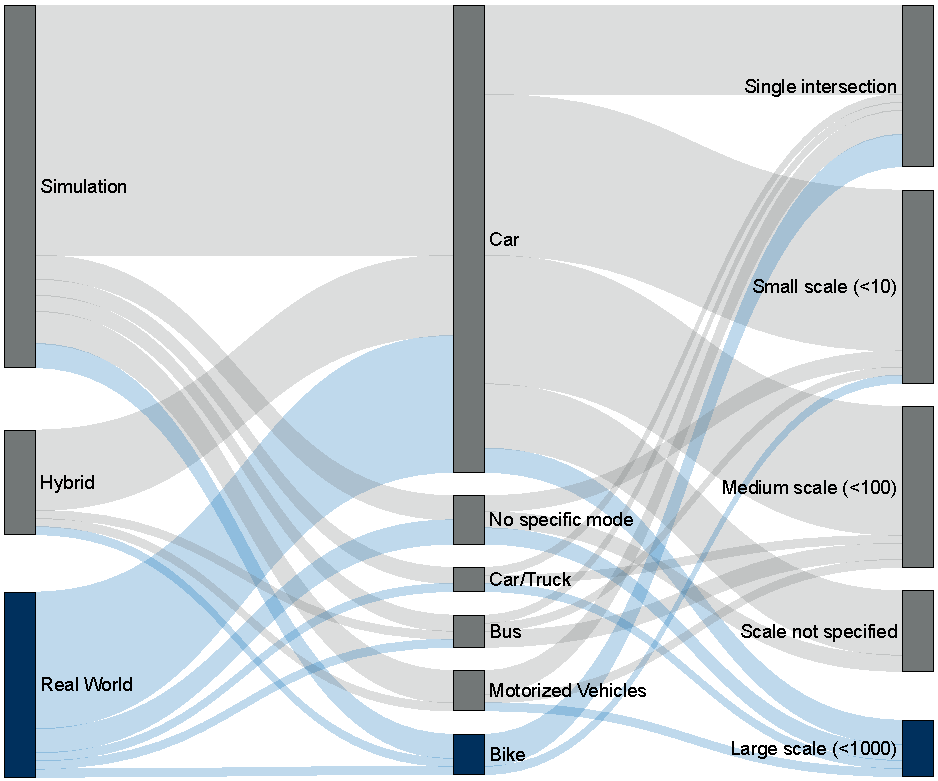
\includegraphics[width=\linewidth]{images/related-work-sankey.pdf}
\caption{Study environment, mode of transport, and number of intersections of related work on GLOSA. Aspects on which this study focuses are highlighted in blue.}
\label{fig:related-work-piechart}
\end{figure}

A key driver in research of GLOSA has been the studies by Audi and BMW, who, from 2008 to 2018, investigated GLOSA in real-world settings as part of their advanced driver assistance systems. In 2014, Protschky et al. \cite{protschky_extensive_2014, protschky_adaptive_2014} focused on a large-scale deployment in Munich, laying the methodological foundation for BMW's "EnLighten" app that was developed later by Wilson et al. (2017) \cite{wilson_driver_2017} and Sokolov et al. (2018) \cite{sokolov_effects_2018}. Both studies were conducted in the USA. In the project TRAVOLUTION (2008) \cite{braun_travolution-netzweite_2009}, Audi collaborated with the city of Ingolstadt and the German firm Gevas to lay the foundation for their own GLOSA system. The system design and the first results were published in 2013 by Zweck and Schuch \cite{zweck_traffic_2013}. By that time, Audi's GLOSA system included the cities of Verona, Garmisch, and Berlin, with a total number of over 700 intersection nodes. Later, in 2017, Stahlmann et al. \cite{stahlmann_multi-hop_2017} investigated options for Audi to directly obtain the traffic light data via short-range radio communication. Finally, in 2018, Stahlmann et al. \cite{stahlmann_exploring_2018} published a paper more broadly focusing on practical problems, finding that there are still unsolved challenges, even though development on GLOSA had proceeded for a decade at this point.

All of these studies have been tested in relatively extensive areas, enabled through the initiatives and pilots brought forward by car manufacturers in collaboration with cities. Apart from these studies, only a few works have investigated GLOSA on a similar scale. Khan et al. (2021) \cite{khan_eco-drive_2021} develop a cloud-based ECO-Driving system for the city of Ottawa with access to 1178 intersections. Bhattacharyya et al. (2022) \cite{bhattacharyya_assessing_2022} utilize data from a field-operational test in Bordeaux with access to 546 intersections. The work by Bhattacharyya et al. (2022) \cite{bhattacharyya_assessing_2022} is related to the mobile apps "CTD - Mobilité connectée"\footnote{\url{https://play.google.com/store/apps/details?id=com.geolocsystems.cthedifference}}, "CoopITS"\footnote{\url{https://play.google.com/store/apps/details?id=fr.gouv.developpementdurable.coopits}}, and work on the Cooperative Urban Mobility Portal\footnote{\url{https://co-ump.eu/data-samples-glosa/}} for Bordeaux. Two other commercial apps were developed in Germany: "TrafficPilot" (available in >10 German cities) by Gevas or "Signal2X" (available in Darmstadt) by Yunex \cite{yunex_traffic_v2x-kommunikation_2023}. Except these projects, most real-world GLOSA studies utilize a testbed with few turns, few traffic lights, and often a predefined route \cite{iglesias_i2v_2008, schweiger_elisatm_2011, raubitschek_predictive_2011, koukoumidis_signalguru_2011, koukoumidis_leveraging_2012, hao_eco-approach_2019, fickas_fast_2019, chen_developing_2022}. City-scale studies are still highly demanded to learn more about the applicability and benefits, but also potential drawbacks of GLOSA to real-world traffic.

Furthermore, research on GLOSA has been traditionally focused on car applications, and only a few studies have focused on transporting the progress in this domain over to cyclists. 

- Tal et al. (2016) \cite{tal_vehicular-communications-based_2016}: mobile system for e-bikes, evaluated in a hybridized simulation environment
- Dabiri et al. (2020) \cite{dabiri_optimized_2020}: optimized speed trajectories (simulation) based on different cyclist preference models -> coping with individuality of cyclists
- Halbach et al. (2021) \cite{halbach_cooperative_2021}: find 


In simulations, Tal et al. (2016) \cite{tal_vehicular-communications-based_2016}, Dabiri et al. (2020) \cite{dabiri_optimized_2020} and Halbach et al. (2021) \cite{halbach_cooperative_2021} found that cyclists could expect similar improvements in ride comfortability and reduced energy expenditure due to lesser stopping.

The only real-world study of a GLOSA app for cyclists was conducted from 2018 to 2021 by Fickas and Schlossberg. The developed app, "FastTrack," was tested in 2019 on a small-scale test corridor (6 intersections) in Oregon \cite{fickas_fast_2019}. Auxiliary material on this study is available through the Portland State University online library \cite{fickas_green_2021, fickas_using_2021, fickas_riding_2019, fickas_data_2021, fickas_project_2018}. Apart from mobile apps like TrafficPilot that offer a cyclist mode besides their main application for cars, no other studies investigate GLOSA as a solution to motivate more people to cycle.

In the real world, static info boards were studied to inform cyclists about upcoming green phases \cite{lu_enhancement_2018}. 

In essence, this work aims to bridge the gap between GLOSA's current state -- largely concentrated on motorized vehicles -- and its potential application to a complete city network, with a spotlight on cyclists. The unique challenges posed by this expansive scope necessitate reevaluating established concepts and solutions, ensuring the development of a holistic GLOSA system.

\section{Challenges}

Apart from the general problem of the lack of focus on cyclists, the research domain surrounding GLOSA raises many interdisciplinary research issues: regulation and financing, integration and technology assessment, and possible consequences for society. This work focuses on the technical implementation of such a system and its assessment, resulting in four problems to address.

\addcontentsline{toc}{subsection}{Traffic Light Data for Prediction}
\textbf{\color{cidarkblue}Traffic Light Data for Prediction:} To provide a speed advisory for an upcoming traffic light, a prediction of the traffic light's switching behavior is required. The challenge lies in developing a robust system that is capable of seamlessly collecting real-time data from traffic lights across the city. This involves not only the integration of a data source but also the implementation of a prediction algorithm that can incorporate the recorded data and forecast the traffic light's behavior. Since a traffic light's switching behavior may depend highly on the current time and day, as well as the detected traffic density, a reliable and accurate prediction is challenging. Furthermore, there may be data outages or errors in the streamed data, which degrade the quality and trustworthiness of the prediction. Hence, achieving a highly accurate and trustworthy prediction is challenging but unquestionably paramount for the overall effectiveness of the speed advisory.

\addcontentsline{toc}{subsection}{Traffic Light Matching}
\textbf{\color{cidarkblue}Traffic Light Matching:} For which traffic light a speed advisory should be displayed depends on the user's planned trajectory across the next intersection(s). The extensive number of potential traffic lights across the city complicates the process, turning the identification of the matching traffic lights into a search for needles in the haystack. The system needs to efficiently and accurately pinpoint the relevant traffic lights that align with the user's route, considering factors such as distance and turn direction. The type of traffic traffic light is also important since cyclists occasionally share a traffic light with cars, buses, or pedestrians. The system should prefer dedicated traffic lights for cyclists whenever possible. Due to the often ambiguous choice in traffic lights at an intersection, the matching algorithm has to consider multiple variants and decide on the best traffic light. The challenge here lies not only in the algorithmic complexity of traffic light matching but also in ensuring real-time responsiveness to provide timely speed advisories.

\addcontentsline{toc}{subsection}{Accurate Bike Routing}
\textbf{\color{cidarkblue}Accurate Bike Routing:} To know which traffic lights will be along the way, this work will utilize a route-based approach for trajectory prediction and distance-to-signal estimation. This means that calculating a route accurately resembling bike trails is crucial for the speed advisory's accuracy. However, existing routing foundations are designed as general-purpose maps with a focus on motorists, meaning that bike paths are often missing or tagged inconsistently. One key focus of this work is, thus, to find methods that allow a more accurate bike routing to enhance the overall in-app experience and provide a solid foundation for an accurate speed advisory.

\addcontentsline{toc}{subsection}{Speed Advisory}
\textbf{\color{cidarkblue}Speed Advisory:} As cyclists navigate with the GLOSA app through the urban landscape, it becomes essential to tailor speed advisories to their individual needs and the context of their journey. This involves reducing cognitive load on the user as much as possible, allowing the cyclist to focus on the real-world situation. Maximizing the usefulness of the advisory system involves striking a balance between providing targeted speed advisories and avoiding unnecessary distractions. Factors such as the road's inclination, surface quality, and the type of bike being used are also crucial to determining the best route and speed advisory. Having solved these challenges, we can deploy the mobile application in a large-scale context and evaluate its impact. One major challenge is finding metrics that decrypt the recorded user data into meaningful insights about the impact of GLOSA on cycling behavior. A multifaceted approach is necessary to tackle this, encompassing quantitative and qualitative data. Understanding user perspectives is vital for ensuring that GLOSA aligns with user expectations and integrates seamlessly into their cycling routines. 

Together, these challenges represent the framework for this work to demystify the overarching question of how well the idea of GLOSA adapts to cyclists in a large-scale, real-world setting. By addressing one challenge by one, this study aims to draw potential repercussions and future work of implementing GLOSA for cyclists.

\section{How to Read This Thesis}

Having discussed the top-level structure and motivation of this work, the rest of this work is structured as follows. Each chapter follows one described challenge along the processing chain of a GLOSA system. First, in \Cref{ch:prediction}, we will discuss the challenge of traffic light prediction, contributing to the understanding of traffic light switching patterns and real-world deployment challenges, and obtaining a functional city-scale prediction system for our bike-GLOSA app. Afterward, in \Cref{ch:matching}, we connect the traffic light prediction with the cyclist by allowing the cyclist to match traffic lights along a preselected route. In \Cref{ch:routing}, we develop an accurate bike routing that improves traffic light matching and distance-to-signal estimation. The routing is integrated together with traffic light prediction and matching into the bike-GLOSA app in \Cref{ch:app}, focusing on the user interface to provide the best possible speed advisory. In this chapter, we also evaluate the impact of the speed advisory on cyclist behavior. 

Each chapter is self-contained and can also be read separately. In each chapter, a more challenge-specific introduction is given, delving into a report of current related work and observed research gaps. The described research gaps are described alongside methods to address these gaps. Finally, these methods are evaluated to draw conclusions and future avenues for research. Small summaries are given at the end of each section that provide all key points. At the end of this thesis, \Cref{ch:conclusions} summarizes the gained knowledge and main results for all individual challenges and gives an overarching outlook for future studies. 
